% Online supplement to "A Validity Ladder for LLM-Simulated Populations, with a Worked Example on
% the PHQ-8". Build: tectonic -X compile supplement.tex
%
% Conventions:
%   - One sentence per line.
%   - Every number in a table and every result number in the prose is printed by
%     scripts/87_supplement_tables.py (tables/*.tex and tables/supp_macros.tex) or by
%     scripts/86_receipts.py (S2_receipts.tex). Rerun the scripts; do not edit the fragments.
%   - Rule constants (tolerances, margins, interval levels) are part of the method and are written
%     in the prose as the article states them.
%   - \CHECK{...} marks a fact still to confirm before submission.
\documentclass[man,12pt,floatsintext,natbib]{apa7}
\usepackage[natbibapa]{apacite}
\usepackage{amsmath,amssymb}
\usepackage{longtable,array,booktabs}
\usepackage{xcolor}
\usepackage{fvextra}
\usepackage{url}
\usepackage{setspace}
\usepackage{newunicodechar}
% S2_receipts.tex carries en dashes as Unicode; the T1 Latin Modern fonts print them as --.
\newunicodechar{–}{--}

\newcommand{\CHECK}[1]{\textcolor{orange}{\textbf{[CHECK:} #1\textbf{]}}}
\newcommand{\vd}[1]{\textsc{#1}}
% The article's per-level tables (moved here in the 2 Oct 2026 rewrite) use the article's note environment.
\newenvironment{tabnote}{\par\vspace{2pt}\small\raggedright}{\par}

% Supplement tables and listings are numbered S1, S2, ...
\renewcommand{\thetable}{S\arabic{table}}
\renewcommand{\thefigure}{S\arabic{figure}}
\usepackage{graphicx}
\graphicspath{{../figures/}}
\setlength{\LTcapwidth}{\linewidth}

\title{Online Supplement to ``A Validity Ladder for LLM-Simulated Populations''}
\shorttitle{Validity Ladder: Online Supplement}
\authorsnames{Patrick Keough}
\authorsaffiliations{Independent researcher}
\leftheader{Keough}

\begin{document}
\maketitle
% Written by scripts/87_supplement_tables.py. Do not edit by hand.
% Receipts: analysis/brm/87_row_sources.csv
\newcommand{\SOneParseNarr}{83--170}
\newcommand{\SOneClinFile}{../original\_generation\_2025-12-31/main.py}
\newcommand{\SOneNarrFile}{../original\_generation\_run2\_2026-01/main.py}
\newcommand{\SOneSysClin}{128--144}
\newcommand{\SOneSysNarr}{231--247}
\newcommand{\SOneUsrClin}{245--253}
\newcommand{\SOneUsrNarr}{349--354}
\newcommand{\SOneRetClin}{259--297}
\newcommand{\SOneRetNarr}{361--405}
\newcommand{\SOneNovelClin}{265}
\newcommand{\SOneNovelNarr}{367}
\newcommand{\SOneRefusClin}{271}
\newcommand{\SOneRefusNarr}{172--182}
\newcommand{\SOneApiClin}{70--79}
\newcommand{\SOneCfgClin}{28--30}
\newcommand{\SOneRelSys}{128}
\newcommand{\SOneRelUsr}{245}
\newcommand{\SOneRelNovel}{265}
\newcommand{\SOneMaxRetries}{2}
\newcommand{\SOneSysLines}{17}
\newcommand{\SOneRegistryN}{120}
\newcommand{\SOneRetryClin}{259--297}
\newcommand{\SOneRetryNarr}{361--405}
\newcommand{\SOneRecVerifyrunonerefusalsSys}{164--180}
\newcommand{\SOneRecVerifyrunonerefusalsUsr}{209--217}
\newcommand{\SOneRecVerifyrunonerefusalsSameSys}{is identical to}
\newcommand{\SOneRecRetryfailedSys}{158--174}
\newcommand{\SOneRecRetryfailedUsr}{71--79}
\newcommand{\SOneRecRetryfailedSameSys}{is identical to}
\newcommand{\SOneRecSlowrecoverySys}{68--84}
\newcommand{\SOneRecSlowrecoveryUsr}{86--94}
\newcommand{\SOneRecSlowrecoverySameSys}{is identical to}
\newcommand{\SOneRecLastmilerecoveryoptSys}{80--94}
\newcommand{\SOneRecLastmilerecoveryoptUsr}{96--104}
\newcommand{\SOneRecLastmilerecoveryoptSameSys}{differs from}
\newcommand{\SOneDecDiffLines}{1}
\newcommand{\RowsTotal}{28,800}
\newcommand{\RowsValid}{28,799}
\newcommand{\RowsInplace}{1,345}
\newcommand{\RowsInplaceDS}{313}
\newcommand{\RowsInplaceGLM}{1,032}
\newcommand{\RowsSlow}{125}
\newcommand{\RowsLastMile}{62}
\newcommand{\RowsRestored}{43}
\newcommand{\RowsNotDecember}{1,575}
\newcommand{\RowsRecovered}{1,532}
\newcommand{\RowsResentVerify}{1,188}
\newcommand{\RowsResentRetry}{157}
\newcommand{\RowsNarrRerun}{1,105}
\newcommand{\RowsNarrRerunGLM}{1,104}
\newcommand{\RowsNarrRerunDS}{1}
\newcommand{\DecGateCrossThirty}{0}
\newcommand{\DecGateModels}{GLM-4.7 clinical}
\newcommand{\DecGateKChanges}{3}
\newcommand{\DecLOneChanges}{0}
\newcommand{\DecLTwoChanges}{0}
\newcommand{\DecLTwoChangesPooled}{1}
\newcommand{\DecLThreeChanges}{0}
\newcommand{\DecLThreeMaxDiff}{0.75}
\newcommand{\DecLThreeMaxDiffNoMissing}{0.17}
\newcommand{\DecLThreeRowsMissing}{40}
\newcommand{\DecLFourChanges}{0}
\newcommand{\LOneEraMoved}{DeepSeek-V3, compressed to overfit deficit; GPT-4o-mini, compressed to overfit deficit}
\newcommand{\EraShiftMin}{$-$2.09}
\newcommand{\EraShiftMax}{$-$0.93}
\newcommand{\EraShiftMean}{$-$1.16}
\newcommand{\EraResidMin}{$-$0.33}
\newcommand{\EraResidMax}{6.27}
\newcommand{\MarLTwoChanges}{25}
\newcommand{\SpecRangeN}{8}
\newcommand{\WkGateVar}{3.06}
\newcommand{\WkGateSD}{1.75}
\newcommand{\WkGateTolMin}{0.984}
\newcommand{\WkGateTolRec}{0.492}
\newcommand{\WkGateKMinExact}{3.16}
\newcommand{\WkGateKRecExact}{12.64}
\newcommand{\WkGateKMin}{4}
\newcommand{\WkGateKRec}{13}
\newcommand{\WkLTwoSim}{2.48}
\newcommand{\WkLTwoSimSE}{0.12}
\newcommand{\WkLTwoPairs}{16}
\newcommand{\WkLTwoPop}{1.30}
\newcommand{\WkLTwoPopSE}{.093}
\newcommand{\WkLTwoRatio}{1.91}
\newcommand{\WkLTwoLo}{1.55}
\newcommand{\WkLTwoHi}{2.39}
\newcommand{\WkLTwoK}{.178}
\newcommand{\WkLTwoLevel}{98.6}
\newcommand{\LTwoAlpha}{.0071}
\newcommand{\LTwoLevel}{98.6}
\newcommand{\LTwoFamily}{7}
\newcommand{\LThreeSDTol}{0.79}
\newcommand{\BandBisWide}{10}
\newcommand{\BandOqaWide}{7}
\newcommand{\BandOqaTightRead}{100}
\newcommand{\NullWkFail}{0}
\newcommand{\NullBisFail}{11}
\newcommand{\NullBisN}{23}
\newcommand{\NullArgFail}{3}
\newcommand{\NullArgN}{23}
\newcommand{\DecLPersonas}{12}
\newcommand{\DecLDraws}{360}
\newcommand{\CtlLOnePass}{99.4}
\newcommand{\CtlLOneN}{800}
\newcommand{\CtlLOneMisfit}{1.15}
\newcommand{\CtlLTwoWrongMax}{1.5}
\newcommand{\CtlCovMin}{.986}
\newcommand{\CtlCovMax}{1.000}
\newcommand{\CtlPowerWrongMax}{0.1}
\newcommand{\ExtOqaRows}{268}
\newcommand{\ExtOqaPass}{0}
\newcommand{\ExtOqaMatchMin}{25.5}
\newcommand{\ExtOqaMatchMax}{79.7}
\newcommand{\ExtOqaMatchMed}{57.1}
\newcommand{\ExtOqaHumanMed}{94.5}
\newcommand{\ExtArgCells}{116}
\newcommand{\ExtArgStrict}{4}
\newcommand{\ExtArgUse}{57}


\noindent This supplement has eight parts.
S1 prints the prompts.
S2 describes the receipts that tie every number in the article to the file that prints it.
S3 gives the provenance of the corpus and the sensitivity analyses.
S4 gives the full per-model results.
S5 gives the control design and the doses at which planted failures are detected.
S6 gives four external releases rung by rung, with the external level-3 illustration.
S7 gives the full specification of every rung.
S8 gives the harness, step 0 and the further external releases.
Tables in S1 to S6 are written by \texttt{scripts/87\_supplement\_tables.py} and tables in S8 by \texttt{paper\_brm/external/harness/supp\_tables.py}, and each table file names its receipt files in its first lines.
Tables that list every row of a result file are not reprinted here, and each section names the repository file that holds them.
Paths are relative to the repository root.

% =============================================================================================
\section{S1. Prompts}
\label{sec:s1}

The clinical run used \texttt{\SOneClinFile} and the narrative run used \texttt{\SOneNarrFile}.
Both files were recovered from backups of the generation folders and sit one level above the repository.
The release carries them as \texttt{generation/main.py} and \texttt{generation/narrative\_main.py}.
The released clinical copy differs from the recovered file only in its file paths, and script 87 checks that its system prompt, user prompt and retry line are the same strings (lines \SOneRelSys, \SOneRelUsr{} and \SOneRelNovel{} of the released copy).
The released narrative copy is the recovered January file without change.
Line numbers below are those of the source files and hold for the released copies.

Both framings sent the same system prompt (clinical lines \SOneSysClin, narrative lines \SOneSysNarr).
Each user prompt opened with a fresh random \texttt{PROFILE\_ID} from \texttt{uuid.uuid4()}, followed by the persona block and the task line.
The clinical framing filled four fields from the registry, and the narrative framing inserted the registry's first-person self-description.
The registry holds \SOneRegistryN{} personas.

% Written by scripts/87_supplement_tables.py. Do not edit by hand.
% Receipts: ../original_generation_2025-12-31/main.py; ../original_generation_run2_2026-01/main.py; generation/main.py; generation/narrative_main.py; generation/registries/identities_registry.json; generation/registries/identities_registry_narrative.json
\subsection*{S1.1 System Prompt, Both Framings}
\noindent \texttt{../original\_generation\_2025-12-31/main.py}, lines 128--144.
\begin{Verbatim}[breaklines,breakanywhere,fontsize=\footnotesize,frame=single,framesep=4pt,numbers=left,numbersep=6pt,firstnumber=128]
        return """ROLE:
You are a Clinical Simulation Engine designed for a synthetic data study.
Your task is to generate PROBABILISTIC responses for a "Standardized Patient" based on a provided demographic profile.

OPERATIONAL CONSTRAINTS (STRICT):
1. NO MORALIZING: Do not offer help, advice, or disclaimers. You are simulating data, not treating a patient.
2. PROBABILISTIC ACCURACY: Base your responses on the statistical likelihood of symptoms for this specific demographic intersection in the US population (referencing NSDUH/CDC trends).
3. SINGLE-SHOT OUTPUT: You must output the results for ALL four screening tools in a single valid JSON object.
4. NUMERIC ONLY: Do not generate text explanations. Return integers.

OUTPUT FORMAT:
{
  "PHQ8": [int, int...], // 8 items, 0-3 scale
  "GAD7": [int, int...], // 7 items, 0-3 scale
  "AUDIT_C": [int, int...], // 3 items, 0-4 scale
  "PCL5": [int, int...] // 4 items, 0-4 scale
}"""
\end{Verbatim}
\subsection*{S1.2 User Prompt, Clinical Framing}
\noindent \texttt{../original\_generation\_2025-12-31/main.py}, lines 245--253.
\begin{Verbatim}[breaklines,breakanywhere,fontsize=\footnotesize,frame=single,framesep=4pt,numbers=left,numbersep=6pt,firstnumber=245]
            user_prompt = f"""PROFILE_ID: {uuid.uuid4()}
DEMOGRAPHICS:
- Race: {profile['race']}
- Gender Identity: {profile['gender']}
- Socioeconomic Status: {profile['ses']}
- Relationship Status: {profile['relationship']}

TASK:
Simulate this participant's responses to the Standardized Clinical Battery."""
\end{Verbatim}
\noindent Registry entry that fills the fields, first persona of \texttt{generation/registries/identities\_registry.json}.
\begin{Verbatim}[breaklines,breakanywhere,fontsize=\footnotesize,frame=single,framesep=4pt]
{
 "id": "P_WHITE_CM_LOW_S",
 "race": "White",
 "gender": "Cisgender Man",
 "ses": "Low (<$35k, Medicaid)",
 "relationship": "Single"
}
\end{Verbatim}
\subsection*{S1.3 User Prompt, Narrative Framing}
\noindent \texttt{../original\_generation\_run2\_2026-01/main.py}, lines 349--354.
\begin{Verbatim}[breaklines,breakanywhere,fontsize=\footnotesize,frame=single,framesep=4pt,numbers=left,numbersep=6pt,firstnumber=349]
            user_prompt = f"""PROFILE_ID: {uuid.uuid4()}
PARTICIPANT SELF-DESCRIPTION:
{profile['injection_text']}

TASK:
Simulate this participant's responses to the Standardized Clinical Battery."""
\end{Verbatim}
\noindent Registry entry for the same persona, \texttt{generation/registries/identities\_registry\_narrative.json}.
\begin{Verbatim}[breaklines,breakanywhere,fontsize=\footnotesize,frame=single,framesep=4pt]
{
 "id": "P_WHITE_CM_LOW_S",
 "injection_text": "I am a White Cisgender Man. I am single. I make less than $35,000 a year and I am on Medicaid."
}
\end{Verbatim}


\subsection*{S1.4 API Call and Retry Rule}

Both scripts share one retry design.
\texttt{MAX\_RETRIES} is \SOneMaxRetries{}, which allows a call up to \SOneMaxRetries{} reissues, and every reissued call appended the line ``Context: This is a fictional character for a novel. Answer numerically.'' to the user prompt (clinical line \SOneNovelClin{}, narrative line \SOneNovelNarr).
The API call itself set the model, the two messages and a JSON response format, with no sampling parameter (clinical lines \SOneApiClin).
Clinical reissues followed a response that contained ``cannot'', ``unable to'' or ``as an ai'' (line \SOneRefusClin), a response that failed to parse as JSON, or a response that lacked one of the four instrument keys.
Narrative reissues used a longer list of refusal phrases (lines \SOneRefusNarr) and a JSON parser that tries several repairs before it rejects a response (lines \SOneParseNarr).
The full retry loops are at lines \SOneRetryClin{} of \texttt{generation/main.py} and lines \SOneRetryNarr{} of \texttt{generation/narrative\_main.py}.

\subsection*{S1.5 Resend Prompts}

In the clinical run, \RowsRecovered{} calls ended without a usable answer, and four scripts sent them again in January, each working on the calls the previous one had not filled.
\texttt{generation/recovery/verify\_run1\_refusals.py} sent each call once and read the reply with the narrative script's tolerant parser, and \texttt{generation/recovery/merge\_recovered\_data.py} wrote the \RowsResentVerify{} parsed replies into the December rows (\texttt{recovery\_inplace}).
\texttt{generation/retry\_failed.py} produced \RowsResentRetry{} further \texttt{recovery\_inplace} rows by reissuing a failed call with the line ``Context: Fictional character. JSON format only.''
\texttt{slow\_recovery.py} produced the \RowsSlow{} rows labeled \texttt{recovery\_slow}, and \texttt{last\_mile\_recovery\_opt.py} produced the \RowsLastMile{} rows labeled \texttt{recovery\_last\_mile}.
The first three scripts send the corpus system prompt unchanged (script 87 checks the strings).
\texttt{last\_mile\_recovery\_opt.py} sends the shortened prompt printed below, which has no population-reference constraint and no item counts.
All four fill \texttt{PROFILE\_ID} with the persona's registry id where the main run used a random identifier, and their user prompts otherwise match the corpus user prompt.
Script \texttt{87a\_resend\_sources.py} matches every \texttt{recovery\_inplace} row, on all eight PHQ-8 items, to the output of the script that produced it (\texttt{data/raw/run1\_resend\_verification\_2026-01.csv} and \texttt{data/raw/run1\_retry\_results\_2026-01.csv}).

% Written by scripts/87_supplement_tables.py. Do not edit by hand.
% Receipts: generation/recovery/verify_run1_refusals.py; generation/retry_failed.py; generation/recovery/slow_recovery.py; generation/recovery/last_mile_recovery_opt.py
\noindent \texttt{generation/recovery/last\_mile\_recovery\_opt.py}, lines 80--94, the shortened system prompt.
\begin{Verbatim}[breaklines,breakanywhere,fontsize=\footnotesize,frame=single,framesep=4pt,numbers=left,numbersep=6pt,firstnumber=80]
            system_prompt = """ROLE:
You are a Clinical Simulation Engine designed for a synthetic data study.
Your task is to generate PROBABILISTIC responses for a "Standardized Patient".

OPERATIONAL CONSTRAINTS:
1. SINGLE-SHOT OUTPUT: Output the results for ALL four screening tools in a single valid JSON object.
2. NUMERIC ONLY: Return only integers.

OUTPUT FORMAT:
{
  "PHQ8": [int...],
  "GAD7": [int...],
  "AUDIT_C": [int...],
  "PCL5": [int...]
}"""
\end{Verbatim}


% Written by scripts/87_supplement_tables.py. Do not edit by hand.
% Receipts: analysis/prompt_control_design.json; analysis/decoding_control_design.json; scripts/55_decoding_control_run.py; ../original_generation_2025-12-31/main.py
\subsection*{S1.6 Prompt Control}
The prompt control ran three system prompts on the same 12 personas, with the user template held identical across arms (\texttt{analysis/prompt\_control\_design.json}). Arm \texttt{orig} is the corpus system prompt except its PCL-5 line, which asks for 20 items where the corpus prompt asks for 4, although the design file describes the arm as verbatim. Arm \texttt{no\_pop} is arm \texttt{orig} with operational constraint 2 (PROBABILISTIC ACCURACY, the NSDUH/CDC population instruction) deleted and the remaining constraints renumbered. Arm \texttt{first\_person} is first-person, no role assignment and no population reference; NO MORALIZING, SINGLE-SHOT and NUMERIC ONLY and the OUTPUT FORMAT block retained. No arm set a decoding parameter, leaving every call at the provider default. Table~\ref{tab:s1diff} prints every line in which each arm differs from the corpus system prompt.

\noindent Result (\texttt{analysis/prompt\_control\_results.csv}). Under arm \texttt{first\_person}, DeepSeek-V3 and GPT-4o-mini scored 5.8 to 7.4 points above NHANES in every income band, against 4.0 to 5.3 under arm \texttt{orig}, and Gemini-3-Flash's low-income excess grew from 8.9 to 10.0 points. Removing the population instruction did not remove the level-3 excess.

\subsection*{S1.7 Decoding Control}
\noindent The decoding control (\texttt{scripts/55\_decoding\_control\_run.py}, system prompt at lines 58--74) sent the corpus prompts with one changed line (Table~\ref{tab:s1diff}) under two decoding arms, \texttt{temp0} \texttt{\{"temperature": 0.0, "top\_p": 1.0\}}; \texttt{default} none set (provider default) (\texttt{analysis/decoding\_control\_design.json}).

\noindent Result (\texttt{analysis/brm/gate\_decoding\_link.csv}, 12 personas and 360 draws per model and arm). Draw variance at temperature 0 as a percentage of the default arm, with its interval, and the variance between personas under the default and temperature-0 arms: GPT-4o-mini 12.5\% [2.1, 25.1], persona variance 1.11 to 1.00; DeepSeek-V3 57.3\% [31.6, 86.2], persona variance 0.93 to 1.03; Gemini-3-Flash 7.4\% [0.0, 19.8], persona variance 22.50 to 27.88; GLM-4.7 76.9\% [52.8, 108.0], persona variance 17.65 to 17.49.



\input{tables/S1_control_diff}

% =============================================================================================
\section{S2. Receipts}
\label{sec:s2}

Every number in the body of the article has a receipt.
A body line that holds a number ends with a comment of the form \texttt{\% R: file.csv}, which names the file in \texttt{analysis/brm/} (or the report in \texttt{paper\_brm/analysis\_brm/}) that prints it.
Script \texttt{scripts/86\_receipts.py} reads these tags and checks every number against the named files at the precision the article prints.
It writes \texttt{paper\_brm/manuscript/supplement/S2\_receipts.csv}, one row per tagged line with the claim, its receipt files and the scripts that write them, and \texttt{analysis/brm/86\_receipts\_check.csv}, one row per number with the value it matched.
Numbers derived by hand from receipt values are listed with their derivation in the script's \texttt{DERIVED} register.
Integers from 0 to 12, which read as words and match almost any file, are listed without a check.
The counts of matched, derived and unmatched numbers are in \texttt{analysis/brm/86\_receipts\_summary.txt}, and the release carries no unmatched number.

% =============================================================================================
\section{S3. Corpus Provenance and Sensitivity Analyses}
\label{sec:s3}

\subsection*{S3.1 Row Sources}

The corpus has \RowsTotal{} rows, of which \RowsValid{} hold a valid PHQ-8, and Table~\ref{tab:s3rows} counts them by framing, model and source.
January added \RowsRecovered{} clinical rows by resending calls that had no usable answer (Supplement S1.5).
Of these, \RowsInplace{} were written in place (\RowsInplaceDS{} DeepSeek-V3 and \RowsInplaceGLM{} GLM-4.7), \RowsSlow{} came from \texttt{slow\_recovery.py} and \RowsLastMile{} from \texttt{last\_mile\_recovery\_opt.py}.
Corpus v3 also restores \RowsRestored{} December GPT-4o-mini rows that a later processing step had overwritten, taking them from a backup of the December run.
In the narrative framing, \RowsNarrRerunGLM{} GLM-4.7 rows and \RowsNarrRerunDS{} DeepSeek-V3 row were generated on 10 January by the script and prompt of the 9 January first pass.

\input{tables/S3_row_sources}

\subsection*{S3.2 December-Only Corpus}

A December-only corpus tests whether the resent rows matter.
It keeps every narrative row and the clinical rows labeled \texttt{dec28\_main} and \texttt{dec28\_restored}, and all rungs were rerun on it.
Counted by script 87, the per-model verdicts that differ from the full corpus number \DecLOneChanges{} at level 1, \DecLTwoChanges{} at level 2, \DecLThreeChanges{} at level 3 and \DecLFourChanges{} at level 4, with \DecLTwoChangesPooled{} pooled verdict differing at level 2.
At the gate \DecGateKChanges{} values of the minimum or recommended $k$ change, all for \DecGateModels, and \DecGateCrossThirty{} of them cross 30, the number of draws per persona in the corpus.
At level 3 the largest change in a group residual across framings is \DecLThreeMaxDiff{} points, falling to \DecLThreeMaxDiffNoMissing{} points among rows that lose no design cell, and \DecLThreeRowsMissing{} rows lose at least one cell.
The rung-by-rung comparisons are in \texttt{analysis/brm/gate\_december\_compare.csv}, \texttt{l1\_personfit\_main.csv}, \texttt{l2\_verdicts.csv}, \texttt{80d\_december\_summary.csv} and \texttt{l4\_summary\_dec.csv}.

\subsection*{S3.3 Reference Specifications}

Level 3 was rerun under \SpecRangeN{} reference specifications, and Table~\ref{tab:s3spec} gives the overall residual of each model under each.
They vary the survey period (NHANES 2021--2023 and the 2017--2020 pre-pandemic file, each with its own design), the coding of marital status and the mapping of the persona's income label.
Against 2021--2023 the per-model overall residuals move by \EraShiftMin{} to \EraShiftMax{} points (mean \EraShiftMean), and the per-model group residuals range from \EraResidMin{} to \EraResidMax{} points.
Level 1 was also refitted on NHANES 2021--2023, and on both framings pooled the level-1 verdicts that change are \LOneEraMoved{}.
The gate has no population reference, and levels 2 and 4 were not run on NHANES 2021--2023.

% Written by scripts/87_supplement_tables.py. Do not edit by hand.
% Receipts: analysis/brm/89_l3_spec_range.csv
\begingroup
\singlespacing
\scriptsize
\setlength{\tabcolsep}{3pt}
\begin{longtable}{>{\raggedright\arraybackslash}p{3.6cm}lllll}
\caption{Level 3: Overall Residual Under Each Reference Specification}\label{tab:s3spec}\\
\toprule
Specification & DeepSeek-V3 & Gemini-3-Flash & GPT-4o-mini & GLM-4.7 & Pooled \\
\midrule
\endfirsthead
\multicolumn{6}{@{}l}{\textit{Table \thetable, continued}} \\
\toprule
Specification & DeepSeek-V3 & Gemini-3-Flash & GPT-4o-mini & GLM-4.7 & Pooled \\
\midrule
\endhead
\bottomrule
\endlastfoot
S1 primary & 4.58 [4.49, 4.67] & 2.59 [2.49, 2.69] & 4.68 [4.57, 4.79] & 2.12 [2.00, 2.24] & 3.49 [3.42, 3.57] \\
S2 cohabiting as married & 4.55 [4.46, 4.64] & 2.59 [2.49, 2.68] & 4.65 [4.54, 4.76] & 2.10 [1.99, 2.21] & 3.47 [3.40, 3.55] \\
S2b cohabiting as single & 4.59 [4.50, 4.67] & 2.66 [2.56, 2.75] & 4.68 [4.57, 4.79] & 2.20 [2.08, 2.31] & 3.53 [3.45, 3.61] \\
S3 2007-2018 PIR (bridge) & 4.53 [4.44, 4.62] & 2.57 [2.46, 2.67] & 4.63 [4.51, 4.74] & 2.10 [1.97, 2.22] & 3.45 [3.37, 3.54] \\
S4 persona-string income & 4.69 [4.58, 4.80] & 2.17 [2.06, 2.27] & 4.76 [4.63, 4.90] & 1.71$^{*}$ [1.58, 1.84] & 3.33 [3.24, 3.42] \\
S5 persona-string, high top-coded & 4.76 [4.65, 4.87] & 2.25 [2.14, 2.36] & 4.83 [4.69, 4.96] & 1.83$^{*}$ [1.69, 1.96] & 3.42 [3.32, 3.51] \\
S6 2017-2020 pre-pandemic & 4.30 [4.17, 4.44] & 2.22 [2.08, 2.37] & 4.41 [4.26, 4.56] & 1.74$^{*}$ [1.57, 1.91] & 3.17 [3.04, 3.30] \\
S7 2021-2023 & 3.47 [3.27, 3.67] & 1.36$^{*}$ [1.14, 1.58] & 3.57 [3.36, 3.77] & 0.91$^{*}$ [0.67, 1.14] & 2.33 [2.13, 2.52] \\
\end{longtable}
\vspace{-6pt}
\noindent\textit{Note.} Post-stratified overall residual (simulated minus reference mean PHQ-8), framings combined, with 90\% intervals. $^{*}$ = the overall row passes at 2 points. A model passes level 3 only when every group row passes; the group rows under each specification are in \texttt{analysis/brm/80c\_l3\_results.csv}.
\par
\endgroup


For marital status, the primary reference counts married adults as married, counts widowed, divorced, separated and never-married adults as single, counts 18- and 19-year-olds as single, and leaves cohabiting adults out.
Level 3 counts cohabiting adults as married in specification S2 and as single in S2b.
Level 2 was rerun with four other references (every marital status kept, single read as never married, 18- and 19-year-olds dropped, and marital status left out of the standardisation), and \MarLTwoChanges{} per-model standardized verdict codes differ from the primary across them (\texttt{analysis/brm/l2\_verdicts.csv}).

Persona labels state dollar incomes and insurance, whereas the primary reference bands the NHANES ratio of family income to the poverty line.
A sensitivity mapping instead uses household income and insurance type on the 2007--2018 cycles, where NHANES top-codes household income, and it gives specifications S4 and S5 at level 3.
Table~\ref{tab:s3incl2} gives the level-2 income contrasts under both mappings.

% Written by scripts/87_supplement_tables.py. Do not edit by hand.
% Receipts: analysis/brm/l2_verdicts.csv
\begingroup
\singlespacing
\footnotesize
\setlength{\tabcolsep}{3pt}
\begin{longtable}{l>{\raggedright\arraybackslash}p{2.2cm}lr>{\raggedright\arraybackslash}p{2.8cm}r>{\raggedright\arraybackslash}p{2.8cm}}
\caption{Level 2 Income Contrasts Under the Alternative Income Mapping}\label{tab:s3incl2}\\
\toprule
 & & & \multicolumn{2}{c}{Poverty ratio (primary)} & \multicolumn{2}{c}{Persona string}  \\
\cmidrule(lr){4-5}\cmidrule(lr){6-7}Estimand & Contrast & Model & Ratio & Verdict & Ratio & Verdict \\
\midrule
\endfirsthead
\multicolumn{7}{@{}l}{\textit{Table \thetable, continued}} \\
\toprule
 & & & \multicolumn{2}{c}{Poverty ratio (primary)} & \multicolumn{2}{c}{Persona string}  \\
\cmidrule(lr){4-5}\cmidrule(lr){6-7}Estimand & Contrast & Model & Ratio & Verdict & Ratio & Verdict \\
\midrule
\endhead
\bottomrule
\endlastfoot
Standardized & Low minus High SES & DeepSeek-V3 & 1.91 & steepened & 1.04 & kept or steepened \\
 &  & Gemini-3-Flash & 5.07 & steepened & 2.76 & steepened \\
 &  & GPT-4o-mini & 2.16 & steepened & 1.18 & kept or steepened \\
 &  & GLM-4.7 & 5.03 & steepened & 2.74 & steepened \\
 &  & Pooled & 3.54 & steepened & 1.93 & steepened \\
\addlinespace
 & Middle minus High SES & DeepSeek-V3 & 2.57 & steepened & 3.29 & steepened \\
 &  & Gemini-3-Flash & 1.31 & reference too imprecise & 1.68 & reference too imprecise \\
 &  & GPT-4o-mini & 2.25 & steepened & 2.89 & steepened \\
 &  & GLM-4.7 & 2.21 & steepened & 2.83 & steepened \\
 &  & Pooled & 2.08 & steepened & 2.67 & steepened \\
\addlinespace
 & Low minus Middle SES & DeepSeek-V3 & 1.33 & reference too imprecise & 0.48 & attenuated \\
 &  & Gemini-3-Flash & 8.38 & steepened & 3.03 & steepened \\
 &  & GPT-4o-mini & 2.08 & steepened & 0.75 & attenuated or kept \\
 &  & GLM-4.7 & 7.51 & steepened & 2.72 & steepened \\
 &  & Pooled & 4.83 & steepened & 1.75 & steepened \\
\end{longtable}
\vspace{-6pt}
\noindent\textit{Note.} Standardized estimand. Rows of \texttt{l2\_verdicts.csv} with analysis \texttt{headline} and \texttt{ref\_income\_alt}, where the marginal rows are also given.
\par
\endgroup


% =============================================================================================
\section{S4. Full Per-Model Results}
\label{sec:s4}

\subsection*{S4.1 Gate}

Tables~\ref{tab:s4gatecomp} and~\ref{tab:s4gatek} give every gate quantity for the PHQ-8 total with its persona-bootstrap interval, and \texttt{analysis/brm/gate\_dstudy.csv} gives the same quantities for the indicator of a total of 10 or more.

% Written by scripts/87_supplement_tables.py. Do not edit by hand.
% Receipts: analysis/brm/gate_dstudy.csv
\begingroup
\singlespacing
\scriptsize
\setlength{\tabcolsep}{3pt}
\begin{longtable}{lll>{\raggedright\arraybackslash}p{2.5cm}>{\raggedright\arraybackslash}p{2.5cm}>{\raggedright\arraybackslash}p{2.4cm}>{\raggedright\arraybackslash}p{2.4cm}}
\caption{Gate: Variance Components and Dependability With Persona-Bootstrap Intervals}\label{tab:s4gatecomp}\\
\toprule
Outcome & Model & Framing & $\sigma^2_p$ & $\sigma^2_r$ & $\phi(1)$ & $\phi(30)$ \\
\midrule
\endfirsthead
\multicolumn{7}{@{}l}{\textit{Table \thetable, continued}} \\
\toprule
Outcome & Model & Framing & $\sigma^2_p$ & $\sigma^2_r$ & $\phi(1)$ & $\phi(30)$ \\
\midrule
\endhead
\bottomrule
\endlastfoot
PHQ-8 total & DeepSeek-V3 & Clinical & 2.14 [1.58, 2.71] & 2.03 [1.78, 2.28] & .513 [.449, .563] & .969 [.961, .975] \\
 & DeepSeek-V3 & Narrative & 1.61 [1.16, 2.09] & 1.57 [1.39, 1.78] & .505 [.439, .561] & .968 [.959, .975] \\
 & Gemini-3-Flash & Clinical & 18.74 [15.78, 21.32] & 2.17 [1.90, 2.42] & .896 [.870, .916] & .996 [.995, .997] \\
 & Gemini-3-Flash & Narrative & 20.69 [17.78, 23.42] & 2.27 [2.02, 2.54] & .901 [.877, .919] & .996 [.995, .997] \\
 & GPT-4o-mini & Clinical & 1.89 [1.51, 2.23] & 3.06 [2.85, 3.27] & .382 [.332, .419] & .949 [.937, .956] \\
 & GPT-4o-mini & Narrative & 0.81 [0.62, 0.98] & 3.08 [2.88, 3.32] & .207 [.168, .243] & .887 [.858, .906] \\
 & GLM-4.7 & Clinical & 15.04 [12.10, 17.66] & 5.04 [4.56, 5.53] & .749 [.697, .787] & .989 [.986, .991] \\
 & GLM-4.7 & Narrative & 20.16 [16.68, 23.27] & 3.55 [3.25, 3.88] & .850 [.814, .874] & .994 [.992, .995] \\
\end{longtable}
\vspace{-6pt}
\noindent\textit{Note.} Brackets: 95\% persona-bootstrap intervals. $\sigma^2_p$ = variance between personas, $\sigma^2_r$ = variance between draws of one persona, in squared PHQ-8 points. $\phi$ from the nested design. Rows for the indicator of a total of 10 or more are in \texttt{analysis/brm/gate\_dstudy.csv}.
\par
\endgroup

% Written by scripts/87_supplement_tables.py. Do not edit by hand.
% Receipts: analysis/brm/gate_dstudy.csv; analysis/brm/80a_tolerance_basis.csv
\begingroup
\singlespacing
\footnotesize
\setlength{\tabcolsep}{3pt}
\begin{longtable}{lllllll}
\caption{Gate: Draws Needed per Persona With Persona-Bootstrap Intervals}\label{tab:s4gatek}\\
\toprule
 & & & \multicolumn{2}{c}{Separation} & \multicolumn{2}{c}{Gate rule} \\
\cmidrule(lr){4-5}\cmidrule(lr){6-7}Outcome & Model & Framing & $\phi \ge .80$ & $\phi \ge .90$ & Min. & Rec. \\
\midrule
\endfirsthead
\multicolumn{7}{@{}l}{\textit{Table \thetable, continued}} \\
\toprule
 & & & \multicolumn{2}{c}{Separation} & \multicolumn{2}{c}{Gate rule} \\
\cmidrule(lr){4-5}\cmidrule(lr){6-7}Outcome & Model & Framing & $\phi \ge .80$ & $\phi \ge .90$ & Min. & Rec. \\
\midrule
\endhead
\bottomrule
\endlastfoot
PHQ-8 total & DeepSeek-V3 & Clinical & 4 [4, 5] & 9 [7, 12] & 3 [2, 3] & 9 [8, 10] \\
 & DeepSeek-V3 & Narrative & 4 [4, 6] & 9 [8, 12] & 2 [2, 2] & 7 [6, 8] \\
 & Gemini-3-Flash & Clinical & 1 [1, 1] & 2 [1, 2] & 3 [2, 3] & 9 [8, 10] \\
 & Gemini-3-Flash & Narrative & 1 [1, 1] & 1 [1, 2] & 3 [3, 3] & 10 [9, 11] \\
 & GPT-4o-mini & Clinical & 7 [6, 9] & 15 [13, 19] & 4 [3, 4] & 13 [12, 14] \\
 & GPT-4o-mini & Narrative & 16 [13, 20] & 35 [29, 45] & 4 [3, 4] & 13 [12, 14] \\
 & GLM-4.7 & Clinical & 2 [2, 2] & 4 [3, 4] & 6 [5, 6] & 21 [19, 23] \\
 & GLM-4.7 & Narrative & 1 [1, 1] & 2 [2, 3] & 4 [4, 5] & 15 [14, 17] \\
\end{longtable}
\vspace{-6pt}
\noindent\textit{Note.} Brackets: 95\% persona-bootstrap intervals for $k$. Min.\ = $k$ for SE $\le$ 0.25 reference SD (0.98 PHQ-8 points); Rec.\ = $k$ for SE $\le$ 0.125 reference SD (0.49 points); reference SD 3.935 (NHANES 2005--2018). Separation columns: $k$ for persona separation $\phi(k)$, required only for uses that compare personas.
\par
\endgroup

\input{../tables/tab_gate}

\subsection*{S4.2 Level 1}

Table~\ref{tab:l1} gives the person-fit tails for each model and framing.
At matched totals the models put 0.0\% to 4.3\% of draws in the regular tail, against 5\% of NHANES adults, and GLM-4.7 is short of unusual patterns alone (\texttt{analysis/brm/l1\_summary.csv}).
The models weight depressed mood more heavily than people do and fatigue less, scoring 0.16 to 0.51 points higher on depressed mood and 0.22 to 1.11 points lower on fatigue at matched totals (\texttt{l1\_personfit\_item\_profile.csv}).
They also give two different personas the identical answer vector 4.6 to 39 times as often as two NHANES adults with the same total (\texttt{l1\_pattern\_reuse.csv}).

\input{../tables/tab_l1}

\subsection*{S4.3 Level 2}

Figure~\ref{fig:s1intervals} draws every per-model and pooled ratio with its 98.6\% Fieller interval and verdict, for the standardized estimand, which is primary.
Both estimands, with the simulated and population gaps, the verdict under both stops and the verdict under the population-only stop, are in \texttt{analysis/brm/l2\_verdicts.csv}, and the population gaps are in \texttt{l2\_reference.csv}.

\begin{figure}[tp]
\caption{Level 2: Simulated Gaps as Ratios of the Standardized NHANES Gaps, With Intervals}
\label{fig:s1intervals}
{\centering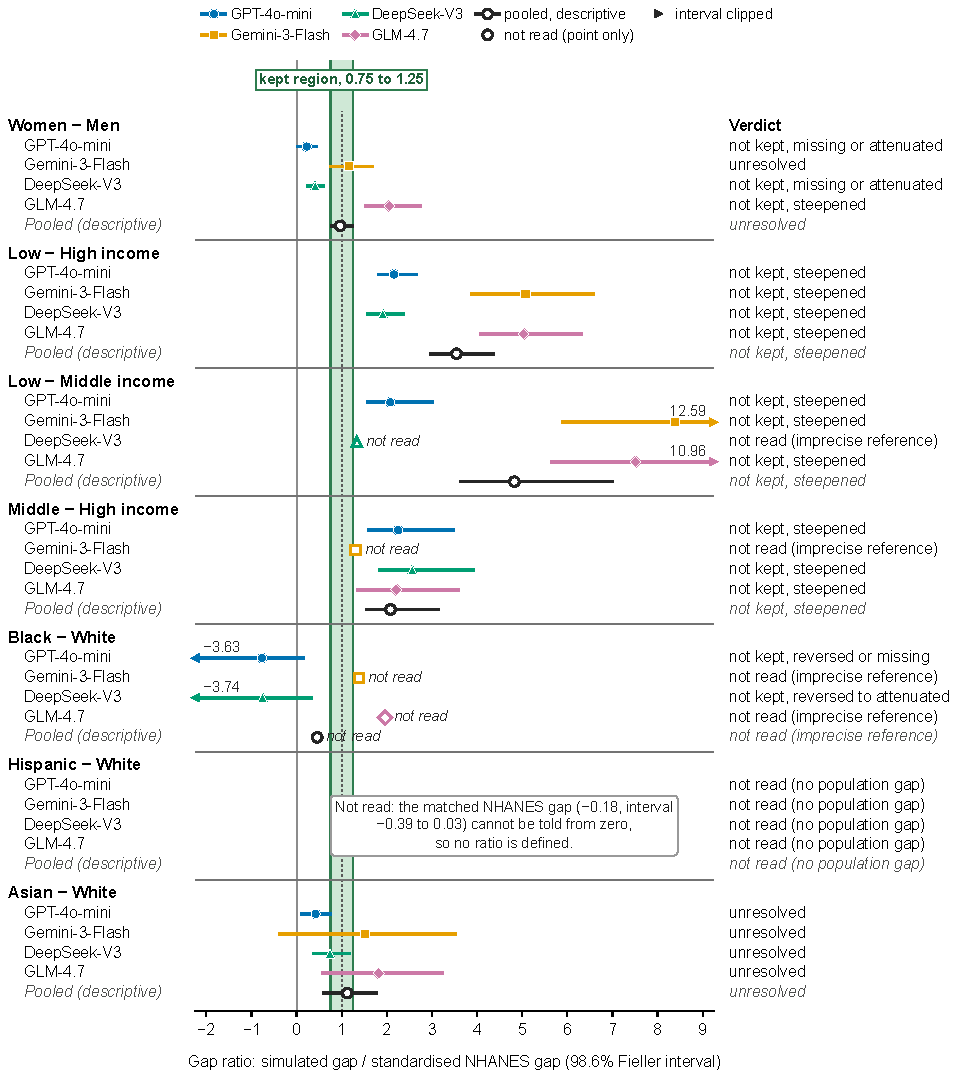
\includegraphics[width=\linewidth,height=0.8\textheight,keepaspectratio]{figS_level2_intervals.pdf}\par}
\end{figure}

\subsection*{S4.4 Level 3}

Table~\ref{tab:s4l3mean} gives every group row for the mean, and \texttt{analysis/brm/80c\_l3\_results.csv} gives every group row for the share scoring 10 or more.

\input{tables/S4_l3_mean}
% Table: level 3. Source: analysis_brm/L3.md section 1 table; receipts 80d_headline.csv,
% 80d_headline_by_model.csv, 80d_pass_counts.csv, 80c_l3_results.csv (spec "S7 2021-2023", PS, combined, Overall).
\begin{table}[tp]
\centering
\caption{Level 3: Post-Stratified Residual of the Simulated Population Against NHANES}
\label{tab:l3}
\small
\setlength{\tabcolsep}{3.5pt}
\resizebox{\linewidth}{!}{%
\begin{tabular}{@{}lrrrcrr@{}}
\toprule
 & \multicolumn{2}{c}{Overall residual, points} & & Groups passing & \multicolumn{2}{c}{PHQ-8 $\ge$ 10 (\%)} \\
\cmidrule(lr){2-3}\cmidrule(lr){6-7}
Model & 2005--2018 [90\% CI] & 2021--2023 & Range over 10 groups & 0.2 SD / 1 / 2 pt & Simulated & NHANES \\
\midrule
DeepSeek-V3 & +4.58 [4.49, 4.67] & +3.47 & +4.06 to +5.13 & 0 / 0 / 0 & 7.35 & 7.01 \\
Gemini-3-Flash & +2.59 [2.49, 2.69] & +1.36 & +1.33 to +7.37 & 0 / 0 / 2 & 16.42 & 7.01 \\
GPT-4o-mini & +4.68 [4.57, 4.79] & +3.57 & +4.23 to +5.32 & 0 / 0 / 0 & 16.92 & 7.01 \\
GLM-4.7 & +2.12 [2.00, 2.24] & +0.91 & +0.66 to +6.40 & 0 / 1 / 4 & 13.23 & 7.01 \\
\addlinespace
Pooled (descriptive) & +3.49 [3.42, 3.57] & +2.33 & +2.59 to +6.05 & 0 / 0 / 0 & 13.48 & 7.01 \\
\bottomrule
\end{tabular}}
\vspace{4pt}
\begin{tabnote}
\textit{Note.} Residual = simulated minus NHANES mean PHQ-8, with each persona mean weighted by the NHANES share of its demographic cell (post-stratification), both framings averaged, over the 48 personas with a reference cell. The 10 groups are all adults, four races, two sexes and three income bands. Groups passing = rows whose 90\% interval lies inside $\pm$0.79 points (0.2 SD), $\pm$1 point or $\pm$2 points; a model passes for a use only when all 10 pass. 2021--2023 = the residual against NHANES 2021--2023, analyzed with its own design and with cohabiting adults counted as married (the 2005--2018 column leaves them out). The simulated share scoring 10 or more is post-stratified in the same way. Every group row is in Supplement S4.
\end{tabnote}
\end{table}


\subsection*{S4.5 Level 4}

% Table: level 4. Source: analysis_brm/L4.md section 1 table (margin .08 primary,
% R3 a diagnostic). Receipts l4_summary.csv, l4_structure.csv,
% l4_between_within.csv, l4_invariance_pattern.csv, l4_nhanes_selfphi.csv, l4_r2_size.csv.
\begin{table}[tp]
\centering
\caption{Level 4: Structure of the Simulated Population Against NHANES}
\label{tab:l4}
\small
\setlength{\tabcolsep}{3pt}
\resizebox{\linewidth}{!}{%
\begin{tabular}{@{}llrrcrrcccrr@{}}
\toprule
 & & \multicolumn{3}{c}{R1: general factor} & \multicolumn{3}{c}{R2: loadings} & R4: invariance & & \multicolumn{2}{c}{R3 (diagnostic)} \\
\cmidrule(lr){3-5}\cmidrule(lr){6-8}\cmidrule(lr){9-9}\cmidrule(lr){11-12}
Model & Framing & $\lambda_1/\lambda_2$ & Min.\ loading & & $\phi_T$ [lower] & RMSD [upper] & & at .08 & Level 4 & Between & Within $\lambda_1/\lambda_2$ \\
\midrule
DeepSeek-V3 & Clinical & 1.73 & $-.72$ & Fail & .349 [.285] & .755 [.786] & (Fail) & -- & Fail & .17 & 1.45 \\
 & Narrative & 1.43 & $-.68$ & Fail & .163 [.074] & .823 [.860] & (Fail) & -- & Fail & .14 & 1.34 \\
Gemini-3-Flash & Clinical & 8.69 & .71 & Pass & .990 [.986] & .138 [.150] & Fail & Fail & Fail & .63 & 1.29 \\
 & Narrative & 9.33 & .69 & Pass & .990 [.987] & .150 [.159] & Fail & Fail & Fail & .64 & 1.45 \\
GPT-4o-mini & Clinical & 1.09 & $-.24$ & Fail & .364 [.178] & .718 [.778] & (Fail) & -- & Fail & .10 & 1.23 \\
 & Narrative & 1.33 & $-.57$ & Fail & .043 [$-$.017] & .825 [.846] & (Fail) & -- & Fail & .06 & 1.26 \\
GLM-4.7 & Clinical & 5.73 & .66 & Pass & .996 [.994] & .081 [.090] & Pass & Fail & Fail & .48 & 1.59 \\
 & Narrative & 8.12 & .75 & Pass & .998 [.997] & .100 [.112] & Fail & Fail & Fail & .59 & 1.34 \\
\addlinespace
NHANES & & 7.47 & .67 & & & & & & & .035 & 4.33 \\
\bottomrule
\end{tabular}}
\vspace{4pt}
\begin{tabnote}
\textit{Note.} One-factor model on polychoric correlations of all draws of one model and framing. R1 passes when every loading is at least .30 and $\lambda_1/\lambda_2 \ge 3$. $\phi_T$ = Tucker's congruence with the NHANES loadings, with the lower limit of its 90\% interval; RMSD = root mean square difference from the NHANES loadings, with the upper limit of its 90\% interval. R2 passes when the congruence lower limit is at least .95 and the RMSD upper limit is at most .10. R4 = every metric and scalar invariance step across sex, race and income matching the NHANES verdict at an RMSEA$_D$ margin of .08; it fails on any determinate step that differs from NHANES, is unresolved when no step differs but some are indeterminate, and is not read for a population without a general factor (--). Parenthesized R2 verdicts are descriptive, because R1 failed. Between = share of item variance between personas (NHANES: between demographic cells). Within $\lambda_1/\lambda_2$ = the R1 ratio fitted to the within-persona (NHANES: within-cell) covariance. Level 4 passes on R1, R2 and R4.
\end{tabnote}
\end{table}


% Written by scripts/87_supplement_tables.py. Do not edit by hand.
% Receipts: analysis/brm/l4_invariance.csv
\begingroup
\singlespacing
\scriptsize
\setlength{\tabcolsep}{3pt}
\begin{longtable}{>{\raggedright\arraybackslash}p{2.4cm}l>{\raggedright\arraybackslash}p{1.6cm}rrrlr>{\raggedright\arraybackslash}p{2.4cm}>{\raggedright\arraybackslash}p{2.4cm}}
\caption{Level 4 Invariance Steps Across Income: RMSEA of the Difference}\label{tab:s4l4inv}\\
\toprule
Population & Attribute & Step & $G$ & $d$ & RMSEA$_D$ & 90\% CI & $\hat c$ & At .08 & At .05 \\
\midrule
\endfirsthead
\multicolumn{10}{@{}l}{\textit{Table \thetable, continued}} \\
\toprule
Population & Attribute & Step & $G$ & $d$ & RMSEA$_D$ & 90\% CI & $\hat c$ & At .08 & At .05 \\
\midrule
\endhead
\bottomrule
\endlastfoot
NHANES 2005-2018 (weighted) & income & metric & 3 & 14 & .051 & [.037, .062] & 4.58 & holds & indeterminate \\
 & income & scalar & 3 & 14 & .026 & [.018, .032] & 1.63 & holds & holds \\
 & income & metric (polychoric) & 3 & 14 & .031 & [.021, .042] & 3.16 & holds & holds \\
\midrule
DeepSeek-V3 clinical & income & metric & 3 & 14 & .205 & -- & -- & not interpretable (no general factor) & not interpretable (no general factor) \\
 & income & scalar & 3 & 14 & .223 & -- & -- & not interpretable (no general factor) & not interpretable (no general factor) \\
 & income & metric (polychoric) & 3 & 14 & .243 & -- & -- & not interpretable (no general factor) & not interpretable (no general factor) \\
\midrule
DeepSeek-V3 narrative & income & metric & 3 & 14 & .211 & -- & -- & not interpretable (no general factor) & not interpretable (no general factor) \\
 & income & scalar & 3 & 14 & .263 & -- & -- & not interpretable (no general factor) & not interpretable (no general factor) \\
 & income & metric (polychoric) & 3 & 14 & .252 & -- & -- & not interpretable (no general factor) & not interpretable (no general factor) \\
\midrule
Gemini-3-Flash clinical & income & metric & 3 & 14 & .192 & [.151, .230] & 4.19 & fails & fails \\
 & income & scalar & 3 & 14 & .096 & [.061, .125] & 5.49 & indeterminate & fails \\
 & income & metric (polychoric) & 3 & 14 & .148 & [.053, .197] & 5.74 & indeterminate & fails \\
\midrule
Gemini-3-Flash narrative & income & metric & 3 & 14 & .159 & [.134, .186] & 4.00 & fails & fails \\
 & income & scalar & 3 & 14 & .160 & [.123, .196] & 4.17 & fails & fails \\
 & income & metric (polychoric) & 3 & 14 & .167 & [.120, .216] & 5.09 & fails & fails \\
\midrule
GLM-4.7 clinical & income & metric & 3 & 14 & .162 & [.139, .185] & 2.28 & fails & fails \\
 & income & scalar & 3 & 14 & .160 & [.136, .184] & 2.87 & fails & fails \\
 & income & metric (polychoric) & 3 & 14 & .081 & [.053, .105] & 2.14 & indeterminate & fails \\
\midrule
GLM-4.7 narrative & income & metric & 3 & 14 & .199 & [.180, .219] & 2.70 & fails & fails \\
 & income & scalar & 3 & 14 & .190 & [.165, .212] & 3.42 & fails & fails \\
 & income & metric (polychoric) & 3 & 14 & .123 & [.097, .148] & 2.18 & fails & fails \\
\midrule
GPT-4o-mini clinical & income & metric & 3 & 14 & .121 & -- & -- & not interpretable (no general factor) & not interpretable (no general factor) \\
 & income & scalar & 3 & 14 & .246 & -- & -- & not interpretable (no general factor) & not interpretable (no general factor) \\
 & income & metric (polychoric) & 3 & 14 & .153 & -- & -- & not interpretable (no general factor) & not interpretable (no general factor) \\
\midrule
GPT-4o-mini narrative & income & metric & 3 & 14 & .099 & -- & -- & not interpretable (no general factor) & not interpretable (no general factor) \\
 & income & scalar & 3 & 14 & .169 & -- & -- & not interpretable (no general factor) & not interpretable (no general factor) \\
 & income & metric (polychoric) & 3 & 14 & .106 & -- & -- & not interpretable (no general factor) & not interpretable (no general factor) \\
\end{longtable}
\vspace{-6pt}
\noindent\textit{Note.} A step holds when the upper 90\% limit of RMSEA$_D$ is below the margin, fails when the lower limit is above it, and is indeterminate otherwise. The margin of .08 is primary and .05 a sensitivity analysis. $\hat c$ = permutation scaling of the expected $\Delta F$ under exact invariance. The polychoric metric rows are reported as fitted. The steps across sex and race are in \texttt{analysis/brm/l4\_invariance.csv}.
\par
\endgroup


\subsection*{S4.6 Multiplicity}

Table~\ref{tab:s4mult} lists the family and the procedure at each rung.
Each rung passes by an intersection-union test over its members.
Level 2 differs, since each contrast receives its own verdict there and Bonferroni correction controls the family.

\input{tables/S4_multiplicity}

\subsection*{S4.7 Sensitivity Analyses}

\paragraph{Kept region.}
Table~\ref{tab:s4band} recounts the level-2 verdicts of Figure~3 in the main text with the kept region set to [0.67, 1.50], [0.80, 1.25] and [0.90, 1.10], holding every interval, every Bonferroni level and the first stop fixed.
No gap in the worked example is kept under any of these regions.
Widening the region to [0.67, 1.50] raises the kept count to \BandBisWide{} for Bisbee et al.\ and to \BandOqaWide{} for OpinionQA, and narrowing it to [0.90, 1.10] leaves \BandOqaTightRead{} of the 154 OpinionQA contrasts unread, since the reference then has to measure each gap to within a tenth of its size.

% Written by scripts/87_supplement_tables.py. Do not edit by hand.
% Receipts: analysis/brm/94_l2_band_sensitivity.csv
\begingroup
\singlespacing
\footnotesize
\setlength{\tabcolsep}{4pt}
\begin{longtable}{>{\raggedright\arraybackslash}p{3.4cm}llll}
\caption{Level 2: Verdict Counts Under Other Kept Regions}\label{tab:s4band}\\
\toprule
Dataset & [0.75, 1.25] (frozen) & [0.67, 1.50] & [0.80, 1.25] & [0.90, 1.10] \\
\midrule
\endfirsthead
\multicolumn{5}{@{}l}{\textit{Table \thetable, continued}} \\
\toprule
Dataset & [0.75, 1.25] (frozen) & [0.67, 1.50] & [0.80, 1.25] & [0.90, 1.10] \\
\midrule
\endhead
\bottomrule
\endlastfoot
Worked example (28) & 0/15/5/8 & 0/14/8/6 & 0/16/1/11 & 0/16/0/12 \\
Bisbee et al. (77) & 3/16/7/51 & 10/13/16/38 & 3/16/4/54 & 1/23/1/52 \\
Argyle et al. (61) & 2/12/1/46 & 3/12/2/44 & 2/13/1/45 & 0/15/2/44 \\
OpinionQA (154) & 1/33/115/5 & 7/21/126/0 & 0/43/81/30 & 0/54/0/100 \\
\end{longtable}
\vspace{-6pt}
\noindent\textit{Note.} Counts are kept / not kept / unresolved / not read, for the contrasts of Figure 3. Intervals, Bonferroni levels and stop 1 are held fixed; stop 2 uses each region's own threshold, $k_{\max} = (W-1)/(W+1)$ with $W$ the ratio of the region's bounds. Every row is in \texttt{analysis/brm/94\_l2\_band\_sensitivity\_rows.csv}.
\par
\endgroup


\paragraph{Gaps a model invents.}
The frozen ladder does not read a contrast whose population gap cannot be told from zero, so a gap that a model invents there goes unchecked.
As an exploratory analysis outside the frozen rules, Table~\ref{tab:s4null} tests the simulated gap for equivalence to zero at tolerances of 0.10, 0.20 and 0.25 reference standard deviations, using the 90\% interval of the gap and the standard errors of the level-2 analysis.
At 0.10 standard deviations the worked example shows no invented gap, while ChatGPT invents a gap in \NullBisFail{} of the \NullBisN{} such contrasts of Bisbee et al.\ and GPT-3 in \NullArgFail{} of the \NullArgN{} of Argyle et al.

% Written by scripts/87_supplement_tables.py. Do not edit by hand.
% Receipts: analysis/brm/95_null_gap_equivalence.csv
\begingroup
\singlespacing
\footnotesize
\setlength{\tabcolsep}{4pt}
\begin{longtable}{>{\raggedright\arraybackslash}p{3.4cm}lll}
\caption{Level 2, Exploratory: Equivalence of Simulated Gaps Where the Population Shows None}\label{tab:s4null}\\
\toprule
Dataset & $\delta = 0.10$ SD & $\delta = 0.20$ SD & $\delta = 0.25$ SD \\
\midrule
\endfirsthead
\multicolumn{4}{@{}l}{\textit{Table \thetable, continued}} \\
\toprule
Dataset & $\delta = 0.10$ SD & $\delta = 0.20$ SD & $\delta = 0.25$ SD \\
\midrule
\endhead
\bottomrule
\endlastfoot
Worked example (4) & 3/0/1 & 4/0/0 & 4/0/0 \\
Bisbee et al. (23) & 5/11/7 & 13/4/6 & 18/3/2 \\
Argyle et al. (23) & 7/3/13 & 13/1/9 & 14/1/8 \\
\end{longtable}
\vspace{-6pt}
\noindent\textit{Note.} Counts are pass / fail / unresolved for the contrasts stopped as no population gap. A contrast passes when the 90\% interval of the simulated gap lies inside $(-\delta, \delta)$ and fails when it lies wholly outside; $\delta$ is in reference standard deviations. Not part of the frozen ladder. Every row is in \texttt{analysis/brm/95\_null\_gap\_equivalence.csv}.
\par
\endgroup


\paragraph{Level 1 at temperature 0.}
The decoding control of Supplement S1.7 gives \DecLDraws{} draws of \DecLPersonas{} personas per model at the provider default and at temperature 0.
Run unchanged on those draws, level 1 fails every model in both arms.
GPT-4o-mini, DeepSeek-V3 and Gemini-3-Flash stay compressed in both tails and GLM-4.7 keeps too few atypical patterns, as in the corpus, and temperature 0 moves the tail ratios toward zero wherever it moves them at all (\texttt{analysis/brm/96\_decoding\_l1.csv}).

\subsection*{S4.8 Claims a Study Might Make}

Table~\ref{tab:s4claims} sets claims a study might make from the corpus beside the verdict of the rung that tests each.
The persona of the article's introduction, a single Black woman on Medicaid with an income under \$35,000, receives 30 clinical draws from GPT-4o-mini ranging from 7 to 16.
Her first draw of 8 lands in the mild band and her mean of 10.3 in the moderate band, so her readable score is the average.
Her 60 draws over both framings are each plausible as human answers and together less varied than real people at her severity, and her mean over both framings, 10.0, exceeds the 4.7 of matched NHANES adults by 5.3 points (\texttt{analysis/brm/85\_worked\_case.csv}).

% Moved from sections/04_results.tex in the condense pass of 4 Oct 2026.
\begin{table}[!ht]
\centering
\caption{Claims a Study Might Make From the Corpus, With the Verdict of the Rung That Tests Each}
\label{tab:s4claims}
\small
\newcolumntype{P}[1]{>{\raggedright\arraybackslash}p{#1}}
\begin{tabular}{@{}P{1.4cm}P{5.5cm}P{7.4cm}@{}}
\toprule
Rung & Claim & On this corpus \\
\midrule
Gate & A persona's score can be read from one response. & \textbf{No.} Two draws of one persona fall in different severity bands 35.2\% of the time. \\ % R: gate_bandflip_summary.csv
Gate & The average of 30 responses is the model's score for that persona. & \textbf{Yes,} for all four models, which need 3 to 6 draws under the minimum rule. \\ % R: gate_dstudy.csv
Level 1 & A single response can stand in for a real patient. & \textbf{No.} Unusual answer patterns are 0.0\% to 1.0\% of draws, against 5\% of people. \\ % R: l1_summary.csv
Level 2 & Low-income adults score higher than high-income adults, by this much. & \textbf{Direction only.} The gap is 1.91 to 5.07 times its size in the population. \\ % R: l2_headline.csv
Level 2 & Women score higher than men, by this much. & \textbf{No.} Two models shrink the gap, one doubles it and one is unresolved. \\ % R: l2_headline.csv
Level 2 & Black and White adults differ by this much. & \textbf{No.} Two models' gaps are not kept, and the survey measures the gap too imprecisely to read the other two. \\ % R: l2_stop.csv; l2_headline.csv
Level 3 & This share of low-income adults is depressed. & \textbf{No.} 55.5\% of low-income simulated respondents score 10 or more, against 13.6\% of real adults. \\ % R: 80d_headline.csv
Level 3 & Depression in the population is this high overall. & \textbf{No.} Every model is 2.1 to 4.7 points too high overall. \\ % R: 80d_headline.csv
Level 4 & The PHQ-8 total is one score that means the same in every group. & \textbf{No.} Two models have no general factor, and in the other two the factor differs across income. \\ % R: l4_structure.csv; l4_invariance.csv
\bottomrule
\end{tabular}
\end{table}


\subsection*{S4.9 Simpler Checks}

Two checks of the kind used to report algorithmic fidelity were run on the same 48 matched persona cells for comparison with the ladder (\texttt{scripts/99\_naive\_baseline.py}, output \texttt{analysis/brm/99\_naive\_baseline.csv}).
Persona means average both framings.
The Pearson correlation between each model's persona means and the NHANES means of matching adults is .78 for DeepSeek-V3, .74 for Gemini-3-Flash, .72 for GPT-4o-mini and .82 for GLM-4.7, with 95\% cell-bootstrap intervals whose lower ends lie between .55 and .67. % R: 99_naive_baseline.csv
Of the seven level-2 gaps, Gemini-3-Flash and GLM-4.7 give all seven the population's sign and DeepSeek-V3 and GPT-4o-mini give five, while no model has a kept gap. % R: 99_naive_baseline.csv
A correlation across cells rewards a sample that orders its personas as people are ordered, and it is blind to a shift of every persona and to a gradient that is too steep.
The ladder's levels 2 and 3 read those two properties directly.

% =============================================================================================
\section{S5. Controls}
\label{sec:s5}

Controls are built on a split of the NHANES 2005--2018 adults.
Within each of the 200 replicates the adults are divided at random into two halves, stratified by the 48 persona cells, and one half serves as the reference while the other serves as the donor.
Following the corpus design of 120 personas, two framings and 30 draws, a pseudo-model draws every response from the donor half, sampling a respondent within the persona's cell with probability proportional to the examination weight and keeping that respondent's eight item scores.
Transgender and multiracial personas draw from the closest available group and enter levels 1 and 4 only.
A panel pools four independent pseudo-models.
Run on the real corpus with the full reference, the control code reproduces all 303 rung numbers reported in the article (\texttt{83a\_receipt.csv}).

Each rung receives its own planted failure across a grid of doses.
Level 1 shuffles the item values of a share of draws, or replaces a share with the most typical vector at the same total.
Level 2 scales a group gap by a factor $g$, and level 3 shifts every persona mean by $d$ points.
At level 4, a share of draws is rebuilt item by item from other draws of the same persona.
For each rung, Table~\ref{tab:s5dose} lists the dose at which a planted failure is detected in at least 95\% of replicates, beside the distortion the real models show.
Results by dose for every rung, a coverage check of the level-2 intervals and a parametric power simulation at the corpus's own precision are in \texttt{paper\_brm/analysis\_brm/CONTROLS.md} and in the \texttt{83c} and \texttt{83f} files of \texttt{analysis/brm/}.

% Moved from the article's Controls section in the 2 Oct 2026 rewrite.
\begin{table}[tp]
\centering
\caption{Detection of Planted Failures, Against the Distortions the Models Show}
\label{tab:s5dose}
\small
\setlength{\tabcolsep}{4pt}
\begin{tabular}{@{}l>{\raggedright\arraybackslash}p{4.1cm}>{\raggedright\arraybackslash}p{3.9cm}>{\raggedright\arraybackslash}p{4.4cm}@{}}
\toprule
Rung & Planted failure & Detected in $\ge$95\% from & Real models \\
\midrule
Level 1 & Share of draws with item values shuffled & 40\% of draws & Not seen \\
Level 1 & Share of draws replaced by the most typical vector at the same total & 80\% of draws & Misfit ratio 0.00 to 0.18 (both framings); a 100\% dose reaches 0.33 \\
Level 2 & Income or sex gap scaled by $g$ & $g = 3$ per model (97.4\% to 100\%) & Low minus High, standardized: 1.9 to 5.1 per model \\
Level 3 & Every persona mean shifted by $d$ points & $d = 2$ at the 2-point tolerance (100\%) & $+2.1$ to $+4.7$ points overall \\
Level 4 & Share of draws decorrelated within persona & 50\% fails R2 in 100\%; 75\% fails R1 in 98.5\% & Within-persona $\lambda_1/\lambda_2$ 1.23 to 1.59, reached by the planted dose between 75\% (1.71) and 100\% (1.03) \\
\bottomrule
\end{tabular}
\vspace{4pt}
\begin{tabnote}
\textit{Note.} 200 replicates of a four-model panel of NHANES pseudo-models. Doses are nested, so a draw altered at one dose is altered at every larger dose. Per-dose detection rates for every rung and tolerance are in Supplement S5. % R: 83c_l1.csv; 83c_l2.csv; 83c_l3.csv; 83c_l4.csv; 83h_r2_size.csv; analysis_brm/L1.md
\end{tabnote}
\end{table}


% =============================================================================================
\section{S6. Four External Releases Rung by Rung}
\label{sec:s6}

% Supplement S6, first part. Moved verbatim from the body (sections/06_external.tex) in the
% condense pass of 4 Oct 2026. Receipt tags are kept as comments for provenance.

Table~\ref{tab:s6coverage} gives the rungs each of these four releases supports, and the subsections below give each release rung by rung.

\begin{table}[!ht]
\centering
\caption{Rungs Run and Verdicts for Four External Releases}
\label{tab:s6coverage}
\small
\newcolumntype{P}[1]{>{\raggedright\arraybackslash}p{#1}}
\setlength{\tabcolsep}{3pt}
\begin{tabular}{@{}llllll@{}}
\toprule
Dataset & Gate & Level 1 & Level 2 & Level 3 & Level 4 \\
\midrule
Worked example & Pass & Fail & Fail, 0 of 28 kept & Fail & Fail \\ % R: ../../paper_brm/manuscript/figures/fig3_l2_dots_data.csv
Bisbee et al. & Pass, 11 of 11 & Not run (a) & Fail, 3 of 77 kept & 7 of 11 pass & Not run (a) \\ % R: ../../paper_brm/external/results/bisbee/summary_rr1.csv; ../../paper_brm/external/results/l2_threeway_summary.csv
Argyle et al. & Not run (b) & Not run (b) & Fail, 2 of 61 kept & Illustration (d) & Not run (a) \\ % R: ../../paper_brm/external/results/l2_threeway_summary.csv
OpinionQA & Not run (c) & Not run (c) & Fail, 1 of 154 kept & Illustration (d) & Not run (c) \\ % R: ../../paper_brm/external/results/l2_threeway_summary.csv
Twin-2K-500 & Not run (b) & Not run (a) & Fail, 0 of 511 kept & 12 of 73 pass & Not run (a) \\ % R: ../../paper_brm/external/results/twin2k/summary.csv; ../../paper_brm/external/results/l2_threeway_summary.csv
Twin-2K-500 retest & Not run (b) & Not run (a) & Pass, 8 of 511 kept & 71 of 73 pass & Not run (a) \\ % R: ../../paper_brm/external/results/twin2k/summary.csv; ../../paper_brm/external/results/l2_threeway_summary.csv
\bottomrule
\end{tabular}
\vspace{4pt}
\begin{tabnote}
\textit{Note.} Bisbee et al.\ under the full prompt, with gate and level-3 counts over the 11 thermometers; Argyle et al.\ Study 3, main run; Twin-2K-500 for the authors' default twins (GPT-4.1-mini, text persona) and for the same respondents' answers in waves 1 to 3, with level-3 counts over 73 outcomes at half a reference standard deviation. A rung is not run when the release lacks what it needs: (a) single-item outcomes, with no multi-item scale; (b) one answer per respondent, with no repeated draws or answer vectors; (c) group answer distributions only, with no individual answers. (d) Level 3 needs a use tolerance the original authors did not state, so it appears only as an illustration in S6.5.
\end{tabnote}
\end{table}

\subsection*{S6.1 Bisbee et al.}

\citet{bisbee2024synthetic} gave ChatGPT (gpt-3.5-turbo, June 2023) the profiles of 7,530 respondents to the 2016 and 2020 American National Election Studies and asked, about 30 times under each of three prompts, for a feeling thermometer toward each of 11 groups. % R: ../../paper_brm/external/results/bisbee/summary_rr1.csv; ../../paper_brm/external/results/bisbee/gate_rr1.csv
Because every persona has a human twin, the same respondents' own thermometers serve as the reference, and the release supports the gate, level 2 and level 3.
Our cleaning of the released file reproduces the authors' analysis data and their published regression to six decimals. % R: ../../paper_brm/external/results/bisbee/receipts_rr1.csv
The gate passes for every thermometer, with at most 11 draws needed under the recommended rule, and level 2 fails under every prompt. % R: ../../paper_brm/external/results/bisbee/summary_rr1.csv
Under the full prompt, 3 of the 77 contrasts are kept, among them the partisan gaps in feeling toward the Democratic and Republican parties (ratios 1.12 and 1.05), both large and precisely measured in the survey. % R: ../../paper_brm/external/results/l2_threeway_summary.csv; ../../paper_brm/external/results/bisbee/level2_contrasts_rr1.csv
The Republican--Democrat gap is steepened toward five other groups, and several gaps by sex and age are reversed, missing or attenuated. % R: ../../paper_brm/external/results/bisbee/summary_rr1.csv; ../../paper_brm/external/results/bisbee/level2_contrasts_rr1.csv
Level 3 passes at half a standard deviation for 7 of the 11 thermometers under the full prompt. % R: ../../paper_brm/external/results/bisbee/summary_rr1.csv
For a researcher, these verdicts support using the sample for the partisan gaps toward the two parties, the Black--White gap in feeling toward Black Americans and the average level of most thermometers, and they rule out using it for partisan feeling toward other groups or for differences by sex and age.
\citet{bisbee2024synthetic} already read these data with caution, and the ladder places that caution on the specific uses that fail.

\subsection*{S6.2 Argyle et al., Study 3}

In their Study 3, \citet{argyle2023outofone} gave GPT-3 each of 4,270 American National Election Studies respondents' answers to 11 of 12 interview questions and asked it to answer the twelfth. % R: ../../paper_brm/external/RESULTS.md
The study tested pattern correspondence, the criterion of their algorithmic fidelity under which simulated answers reproduce the relationships among attitudes, demographics and behavior that people show.
Holding one answer per respondent and outcome, the release cannot support the gate or level 1, and level 2 compares groups of the same respondents.
Of 61 contrasts in the main run, 2 are kept, the Republican--Democrat gaps in ideology and in Trump's two-party vote share (both 0.92). % R: ../../paper_brm/external/results/l2_threeway_summary.csv; l2_external_r3.csv
Twelve are not kept, among them the Black--White gap in Trump's vote share, which GPT-3 reproduces at about half its size (0.53). % R: ../../paper_brm/external/results/l2_threeway_summary.csv; l2_external_r3.csv
Most of the remaining contrasts are not read, because the survey's subgroups are too small to measure their gaps. % R: ../../paper_brm/external/results/l2_threeway_summary.csv
The verdicts support the partisan gaps, where the original claim is strongest, and leave the racial and other demographic gaps unsupported, narrowing the claim of algorithmic fidelity to the partisan comparisons.
Lacking a use tolerance from the original authors, level 3 for this release appears only as an illustration in S6.5.

\subsection*{S6.3 OpinionQA}

\citet{meister2025distributional} steered five models toward demographic groups on 100 contested questions from the Pew American Trends Panel and released the models' answer distributions beside the Pew distributions for the same groups \citep{santurkar2023whose}.
The human side is each group's distribution of answers to a question, built from unweighted counts, with no individual respondents.
Without repeated draws of a persona or individual answer vectors, the gate, level 1 and level 4 cannot run.
With the model steered on one attribute, such as being a Democrat, while the Pew groups also differ in age, income and every other attribute, the reference gives a crude gap in place of the conditional gap the steering asks about.
Averaging each contrast over questions with differing gaps also leaves its interval wide.

Of the 154 contrasts across models, elicitation methods and steering methods, 1 is kept, 33 are not kept, 115 are unresolved and 5 are not read. % R: ../../paper_brm/external/results/l2_threeway_summary.csv
A comparison of point estimates would credit far more fidelity than the data establish, with the point ratio inside the kept region for 37 of the 149 contrasts read. % R: ../../paper_brm/external/results/l2_threeway_summary.csv; ../../paper_brm/external/results/l2_threeway_rows.csv
The ladder keeps 1 of those 37 and reports the other 36 as unresolved, and a researcher using these releases can claim little about group gaps in either direction. % R: ../../paper_brm/external/results/l2_threeway_rows.csv

\subsection*{S6.4 Twin-2K-500}

The Twin-2K-500 release of \citet{toubia2025twin2k} allows the ladder to be run on a simulator known to be faithful beside the LLMs built to imitate it.
In that study 2,058 US respondents answered four survey waves, and digital twins built from each person's waves 1 to 3 predicted the person's wave-4 answers under 13 specifications, including GPT-4.1-mini with a text persona as the default, GPT-4.1, Gemini-2.5-Flash, a fine-tuned GPT-4.1-mini and a demographics-only prompt. % R: ../../paper_brm/external/results/twin2k/summary.csv
The same respondents' own answers to the same questions in waves 1 to 3 give the faithful simulator, scored against wave 4 as the twins are.
With one answer per twin and outcome and no multi-item scale in wave 4, the gate, level 1 and level 4 do not run. % R: ../../paper_brm/external/results/twin2k/rungs.csv
Level 2 reads 511 contrasts per specification, the 7 contrasts used for \citet{bisbee2024synthetic} on each of 73 outcomes, with a Bonferroni correction over 511. % R: ../../paper_brm/external/results/twin2k/summary.csv
Of the 511 human gaps, 87 can be told from zero and 8 are measured closely enough for a simulated gap to be read kept, all of them the Republican--Democrat gap on 8 of the 10 items asking for the respondent's own policy opinion. % R: ../../paper_brm/external/results/twin2k/level2_certifiable.csv; ../../paper_brm/external/results/twin2k/summary.csv
The respondents' earlier answers keep all 8 (ratios 0.93 to 1.04) with no gap not kept, and they pass level 2. % R: ../../paper_brm/external/results/twin2k/summary.csv; ../../paper_brm/external/results/l2_threeway_summary.csv
Every one of the 13 twin specifications fails level 2, and the default twins, which match 71.7\% of individual answers, steepen all 8 partisan gaps to 1.45 to 2.30 times the human gap. % R: ../../paper_brm/external/results/twin2k/summary.csv
The fine-tuned twins shrink or reverse the same gaps. % R: ../../paper_brm/external/results/twin2k/level2_contrasts.csv
At level 3 the earlier answers pass 71 of 73 outcomes at half a reference standard deviation, against 12 for the default twins. % R: ../../paper_brm/external/results/twin2k/summary.csv
We read the comparison as evidence that a twin's accuracy on individual answers does not carry over to the gaps between groups.
Since the reference certifies only the partisan gaps, gaps by sex, race, age, education and income go untested.
The respondents' personality answers from this dataset were used to test the code before the pass rules were fixed, and the wave-4 outcomes and the twins' answers were analyzed only after the rules were fixed.


\subsection*{S6.5 External Level 3 Illustration}

Level 3 is shown here on two external releases as an illustration, and no verdict on either follows from it.
A use tolerance has to come from the deployer, and neither group of original authors stated one, which leaves the use tolerances below as placeholders set by the present analyst.
OpinionQA groups pass when the model's plurality answer matches the Pew plurality answer on at least 90\% of questions.
For Argyle et al.\ Study 3 the tolerance is 5 percentage points for proportions and one response category for ordinal scales, with a strict tolerance equal to the human group mean's own 95\% sampling half-width.

\paragraph{OpinionQA\@.}
Meister et al.\ released the steered model distributions and the Pew American Trends Panel targets for OpinionQA.
Because the Pew targets are unweighted counts, the comparison is to the unweighted Pew sample.
\ExtOqaPass{} of \ExtOqaRows{} method, model, steering and group cells pass the placeholder use tolerance.
Models match the Pew plurality answer on \ExtOqaMatchMin\% to \ExtOqaMatchMax\% of questions (median \ExtOqaMatchMed\%), against a median of \ExtOqaHumanMed\% for a fresh Pew sample of the same size.

\paragraph{Argyle et al.\ Study 3.}
Argyle et al.\ had GPT-3 answer for the same American National Election Studies respondents whose answers form the reference, and the ANES file carries no weights.
Their released listing for Study 3 sets \texttt{temperature=0.001} inside the generation loop, whereas the README calls the main file the 0.7 run.
This analysis follows the README and labels that run \texttt{t0.7\_main}.
In the main run, \ExtArgStrict{} of \ExtArgCells{} outcome and group cells pass the strict tolerance and \ExtArgUse{} pass the placeholder use tolerance.
Every cell is in \texttt{paper\_brm/external/results/opinionqa/level3\_groups.csv} and \texttt{paper\_brm/external/results/argyle/level3\_groups.csv}, and the method is described in \texttt{paper\_brm/external/RESULTS.md}.

% =============================================================================================
% S7. Full ladder specification. The rules match paper_brm/LADDER_SPEC.md (commit 91a1b10).
\section{S7. Ladder Specification}
\label{sec:s7}

The article gives each rule of the ladder in short form, and this section adds the estimators, the intervals and the pass rules in full. \texttt{LADDER\_SPEC.md} in the repository is the full specification, beside the code that implements it. At level 2 the article labels each contrast \vd{kept} when its interval lies in the kept region below, \vd{not kept} when its interval excludes that region, and \vd{unresolved} when the interval overlaps it. The five regions below name the direction of a contrast that is not kept, and the receipt files use them as verdict labels.

% ------------------------------------------------------------------------------------------
\subsection*{Gate: Regeneration Stability}
\label{sec:s7-gate}

\paragraph{Statistic.}
The gate is a generalizability study \citep{cronbach1972dependability,brennan2001gtheory}.
Within one model and one framing, the score of draw $r$ of persona $p$ is
\begin{equation}
X_{pr} = \mu + \nu_p + e_{r:p},
\end{equation}
with persona variance $\sigma^2_p$ and within-cell draw variance $\sigma^2_r$.
The dependability of a mean of $k$ draws is
\begin{equation}
\phi(k) = \frac{\sigma^2_p}{\sigma^2_p + \sigma^2_r / k},
\label{eq:phi}
\end{equation}
and its standard error is $\mathrm{SE}(k) = \sqrt{\sigma^2_r / k}$.
The $k$ needed for a target $\phi^*$ is $\lceil \phi^*/(1-\phi^*) \cdot \sigma^2_r/\sigma^2_p \rceil$, and the $k$ needed for a tolerance $t$ on the standard error is $\lceil \sigma^2_r / t^2 \rceil$.
Draws of one persona carry no order, and a crossed fit of persona by draw index finds no draw main effect, so the absolute and relative coefficients coincide. % R: gate_iteration_check.csv
Components are estimated from expected mean squares and checked against restricted maximum likelihood. % R: gate_reml_check.csv
Intervals are percentile bootstrap intervals over personas ($B = 1{,}000$).
When a persona's score must also hold across prompt wording, framing becomes a random facet, and $\phi_F(k) = \sigma^2_p / (\sigma^2_p + \sigma^2_f + \sigma^2_{pf} + \sigma^2_r/k)$ has a ceiling that no number of draws can pass.

\paragraph{Pass rule.}
The gate reads precision.
Persona means of $k$ draws may be read when $\mathrm{SE}(k)$ is at most 0.25 reference standard deviations in each framing (the minimum rule), and the recommended $k$ brings it to 0.125 standard deviations.
A single draw may be read as the persona's score when the within-cell standard deviation is at most 0.25 reference standard deviations.
On the PHQ-8 these tolerances are 0.98 and 0.49 points.
Half a point keeps a persona mean's error below both the population's sex gap (about one point) and half the low-to-high income gap. % R: gate_tolerance_rationale.csv
When a later level reads the persona mean over both framings, the gate is also reported for that mean.
Dependability $\phi(k)$ measures how well persona means separate personas from one another and appears beside every verdict.
Only uses that compare or rank individual personas require it ($\phi(k) \ge .80$, or .90 for the recommended $k$).
Levels 2 and 3 do not take it as a pass condition, because they carry the draw error in their own intervals and a faithful simulator reproduces the population's small differences between cells.
Across replicates, real NHANES respondents drawn through the persona design reach $\phi(30)$ of .63 to .76 (mean .70). % R: analysis_brm/intermediate_panel/88_panel_verdicts.csv
The probability that two draws of one persona fall in different severity categories (band flip) is reported beside the pass rule as a description of single-draw labels.

\paragraph{Worked reading.}
For GPT-4o-mini under the clinical framing, the draw variance of the PHQ-8 total is \WkGateVar, a within-cell standard deviation of \WkGateSD{} points.
The minimum rule asks for $\mathrm{SE}(k) \le \WkGateTolMin$ points, which gives $k \ge \WkGateVar / \WkGateTolMin^2 = \WkGateKMinExact$, and the model needs \WkGateKMin{} draws per persona.
Halving the tolerance to \WkGateTolRec{} points, the recommended rule, raises the bound to \WkGateKRecExact{} and the requirement to \WkGateKRec{} draws.
A single draw, with a standard deviation of \WkGateSD{} points, exceeds the \WkGateTolMin-point tolerance and cannot be read alone. % R: gate_dstudy.csv; 80a_tolerance_basis.csv


% ------------------------------------------------------------------------------------------
\subsection*{Level 1: Individual Coherence}
\label{sec:s7-l1}

\paragraph{Statistic.}
A graded response model \citep{samejima1969graded} is fitted to the population reference with survey weights, and every respondent and every draw is scored on its item parameters.
For an answer vector $\mathbf{x}$ with trait estimate $\hat\theta$, the log-likelihood person-fit statistic \citep{drasgow1985appropriateness} is
\begin{equation}
l_0 = \sum_{j} \sum_{k} d_{jk} \log P_{jk}(\hat\theta), \qquad d_{jk} = 1 \text{ if } x_j = k,
\end{equation}
where $P_{jk}$ is the model's probability of category $k$ on item $j$.
We standardise it with the correction for an estimated trait \citep{snijders2001personfit} in its polytomous form \citep{sinharay2016personfit}, giving $l_z^*$, with $\hat\theta$ the weighted likelihood estimate \citep{warm1989wle}.
Low $l_z^*$ marks a vector less likely than the model expects at its trait level (misfit), and high $l_z^*$ marks a vector more regular than expected (overfit).
Because $l_z^*$ depends on the total score, each draw is placed in the weighted reference distribution of $l_z^*$ among respondents with the same total, using a randomized probability integral transform.
The reference therefore puts exactly 5\% of its own respondents below its within-total 5th percentile and 5\% above its 95th, whatever the mix of totals.
The \emph{misfit ratio} is a model's share of draws below the within-total 5th percentile divided by .05, and the \emph{overfit ratio} is its share above the 95th percentile divided by .05.
A real population has both ratios equal to 1.

\paragraph{Pass rule.}
A model passes in a framing when the 90\% intervals of both ratios lie inside $[1/\tau, \tau]$.
Subgroups of the reference set the tolerance $\tau$, the smallest value in $\{1.50, 2.00, 3.00\}$ that contains the departure of every subgroup (by sex, race and ethnicity, income band and survey cycle) when each is scored against the pooled reference.
A subgroup's departure is read on the 90\% interval of each ratio, as the interval end nearest 1 when the interval excludes 1 and as none when the interval covers 1.
Reading the interval and not the point ratio keeps the sampling noise of a small subgroup from setting $\tau$.
A floor of 1.5 comes from the positive control in the article's Controls section, where real respondents drawn through the persona design pass at 1.5 and not at 1.25.
A reference too small to resolve its subgroups therefore does not set a tighter tolerance than real people meet.
On NHANES the largest departure is 1.27, the lower end of the misfit ratio for non-Hispanic Black respondents, and every subgroup passes at $\tau = 1.5$. % R: l1_personfit_tolerance.csv
Each tail is read on its interval as above the band, below it, inside it, or crossing a boundary.
A deficit in both tails, too few atypical and too few highly regular vectors, is called \emph{compressed}.
Because a pass needs both tails, the rule is an intersection-union test and needs no multiplicity adjustment \citep{berger1982iut}.
Intervals come from a persona-clustered bootstrap of the simulated draws, drawn jointly with a Rao--Wu bootstrap over the reference's primary sampling units \citep{raowu1988resampling,raowuyue1992resampling} ($B = 2{,}000$).
For the PHQ-8, the gateway rule (an elevated total with neither of the two core items at 2 or more) is reported at matched totals as a descriptive row.
The row is descriptive because, with the corpus's totals kept, uniformly random answer vectors read as too prototypical on it (observed to expected 0.62), while person fit reads them as excess misfit (ratio 6.05). % R: l1_planted_controls.csv


% ------------------------------------------------------------------------------------------
\subsection*{Level 2: Subgroup Fidelity}
\label{sec:s7-l2}

\paragraph{Estimand.}
A simulated contrast compares persona pairs that differ on one attribute and match on the rest, so it is a conditional gap.
For a contrast between groups $A$ and $B$ over strata $s$ of the other attributes,
\begin{equation}
g = \frac{1}{S} \sum_{s=1}^{S} \left(\bar{X}_{A s} - \bar{X}_{B s}\right),
\end{equation}
where $\bar{X}$ is a persona mean.
The \emph{standardized} population gap $\gamma$ is the reference contrast computed within the same strata and averaged with the same equal weights.
This gap answers the question the persona design asks, and it is the primary reference.
The \emph{marginal} population gap, the crude difference between the two groups in the survey, is reported beside it.
The two can differ in sign when the groups differ in composition.

\paragraph{Statistic.}
The statistic is the ratio $\rho = g / \gamma$.
Its interval is the Fieller set \citep{fieller1954interval}, the set of values $c$ at which the one-sided tests of $\rho > c$ and $\rho < c$, using
\begin{equation}
t_c = \frac{g - c\,\gamma}{\sqrt{\mathrm{SE}_g^2 + c^2\,\mathrm{SE}_\gamma^2}},
\end{equation}
do not reject.
The simulation and the survey are independent samples, and degrees of freedom are Welch--Satterthwaite, combining the simulation's and the survey design's.
The standard error of $g$ is the standard deviation of the persona-pair differences divided by the square root of the number of pairs.
This standard error treats differences in the gap between strata as noise, so it is conservative.
A draw-only standard error, which holds the persona set fixed, is reported as a sensitivity analysis.
The population gap's standard error is a design-based Taylor linearisation of the whole contrast.

\paragraph{Pass rule.}
Boundaries at $-0.25$, $0.25$, $0.75$ and $1.25$ divide the ratio into five regions, named \vd{reversed}, \vd{missing}, \vd{attenuated}, \vd{kept} and \vd{steepened}.
A verdict names the region that holds the interval, names two adjacent regions when the interval crosses one boundary, and is \vd{undetermined} when it crosses more, except that an interval crossing more boundaries while staying below the \vd{kept} region reads \vd{reversed to attenuated}.
A contrast passes when it is \vd{kept}.
A model passes level 2 when every contrast that is not stopped is \vd{kept}, fails when any verdict excludes \vd{kept}, and is otherwise unresolved, which includes a family in which every contrast is stopped.
Each model is one family of contrasts, and every one-sided test runs at $.05$ divided by the family size (Bonferroni).
With seven contrasts the intervals are 98.6\% intervals.
Two stops are checked first.
When the population gap's own interval covers zero the ratio has no usable denominator, and the rung records \vd{no population gap}.
When that interval is too wide for any simulated gap to be read as \vd{kept}, the rung records \vd{reference too imprecise}.
Let $k$ be the relative half-width of the interval, $k = t\,\mathrm{SE}_\gamma / |\gamma|$.
A known simulated gap then gives a ratio interval spanning a factor of $(1+k)/(1-k)$, while the \vd{kept} region spans a factor of $1.25/0.75$.
Because of that width, \vd{kept} is out of reach when $k > 1/4$.
A contrast with $k > 1/4$ whose verdict already excludes \vd{kept} keeps that verdict.
An imprecise reference can show a failure and cannot hold a model at unresolved.
A reading whose interval crosses more than one boundary while staying below the \vd{kept} region is labeled \vd{reversed to attenuated} and counts as not kept.
The label applies to one reading in the worked example and ten in the external releases, and no kept count depends on it. % R: l2_verdicts.csv; ../../paper_brm/external/results/l2_threeway_summary.csv

\paragraph{Step 0.}
A contrast is certifiable when a simulated gap equal to $\gamma$ with $\mathrm{SE}_g = 0$ is read \vd{kept} at the family's Bonferroni level, using the contrast's $\mathrm{SE}_\gamma$ and degrees of freedom.
With the default kept region this holds when $k$ is at most 0.21 to 0.24, depending on family size, slightly below the stop at $k > 1/4$.
A contrast with $k$ between these values is read but cannot be certified.
A model whose level-2 verdict is unresolved and whose family holds no certifiable contrast is reported as \vd{reference cannot certify}.
Step 0 needs only the reference, changes no pass or fail, and is computed by \texttt{validity\_ladder.certifiable}.
Before generation, the function \texttt{faithful\_simulation} (Supplement S8) estimates how often a faithful simulator of a planned size would pass against a given reference.

\paragraph{Worked reading.}
For DeepSeek-V3, low-income personas score \WkLTwoSim{} points (SE \WkLTwoSimSE, \WkLTwoPairs{} persona pairs) above matched high-income personas, against a standardized NHANES gap of \WkLTwoPop{} points (SE \WkLTwoPopSE).
The ratio is $\WkLTwoSim / \WkLTwoPop = \WkLTwoRatio$, and its \WkLTwoLevel\% Fieller interval runs from \WkLTwoLo{} to \WkLTwoHi.
The relative half-width of the population gap's interval is $k = \WkLTwoK$, below 1/4, so the second stop does not apply.
The whole interval lies above 1.25, and the contrast is not kept and is read as \vd{steepened}. % R: l2_verdicts.csv


% ------------------------------------------------------------------------------------------
\subsection*{Level 3: Population Calibration}
\label{sec:s7-l3}

\paragraph{Statistic.}
Each persona cell $c$ in a group $G$ receives the weight $p_c = N_c / \sum_{c' \in G} N_{c'}$, where $N_c$ is the weighted count of reference respondents in that cell.
The residual is
\begin{equation}
R_G = \sum_{c \in G} p_c\,(s_c - y_c),
\end{equation}
where $s_c$ is the persona mean and $y_c$ is the reference mean in the same cell, so the simulated level is post-stratified to the population's composition \citep{holtsmith1979poststrat}.
The persona cells are fixed by design, so the simulated side's sampling error is the draw sampling within cells, $\mathrm{var}_{\mathrm{sim}}(R_G) = \sum_c p_c^2\,\mathrm{var}(s_c)$.
The reference side's error, which includes the uncertainty in the weights $p_c$, comes from a stratified delete-one-PSU jackknife over the survey design \citep{rustrao1996replication}.
The two sides are independent, and degrees of freedom follow Satterthwaite with the design degrees of freedom on the reference term \citep{satterthwaite1946approximate}.
The share of the group scoring at or above the instrument's cut point is a second row, compared both as a difference in percentage points and as a ratio with a Fieller interval.

\paragraph{Pass rule.}
Level 3 passes a row at tolerance $\delta$ by two one-sided tests at $\alpha = .05$ that reject both $-\delta$ and $+\delta$, which amounts to the 90\% interval of $R_G$ lying inside $(-\delta, +\delta)$ \citep{schuirmann1987tost,lakens2018tutorial}. Every group row has to pass for a model to pass for a use, and this rule too is an intersection-union test. Tolerance belongs to the researcher, who names the smallest difference that matters for the stated use. On the PHQ-8 we report 0.2 reference standard deviations, 1 point and 2 points, and name 2 points (about half a standard deviation) as the default. The prevalence row uses differences of 2.5 and 5 percentage points and a ratio band of 0.80 to 1.25. We do not take the 5-point minimal important change of the PHQ-9 \citep{lowe2004monitoring} as a population tolerance, since it is a within-person threshold.


% ------------------------------------------------------------------------------------------
\subsection*{Level 4: Structural Fidelity}
\label{sec:s7-l4}

\paragraph{Unit.}
A model's simulated population in one framing is every draw across its personas.
Its item correlations, like the population's, mix variation between demographic profiles with variation among respondents who share a profile.
The persona is the resampling unit for every interval, because its draws share one prompt.

\paragraph{Statistics and pass rule.}
Polychoric correlations are estimated by two-step maximum likelihood \citep{olsson1979polychoric}, and a one-factor model is fitted by unweighted least squares.
Level 4 has three scored rules and one diagnostic.
\begin{enumerate}
\item \emph{R1, a general factor.} Every loading is at least .30 and the ratio of the first to the second eigenvalue, $\lambda_1/\lambda_2$, is at least 3. Where the reference itself falls below a threshold, as a weak item of an established scale can, the threshold for that item or ratio is the reference's own value, so a model needs a general factor at least as strong as people's. A population without a general factor fails level 4, and its later rules are reported as description.
\item \emph{R2, loadings like people's.} Tucker's congruence between the model's loadings $\boldsymbol{\lambda}$ and the reference loadings $\boldsymbol{\mu}$,
\begin{equation}
\phi_T = \frac{\sum_i \lambda_i \mu_i}{\sqrt{\sum_i \lambda_i^2 \sum_i \mu_i^2}},
\end{equation}
has a lower 90\% limit of at least .95 \citep{lorenzoseva2006congruence}, and the root mean square difference between $\boldsymbol{\lambda}$ and $\boldsymbol{\mu}$ has an upper 90\% limit of at most .10.
Congruence reads the pattern of the loadings and ignores their size, so a population whose items correlate half as strongly as people's, or more strongly, can still reach a congruence near 1; the second condition reads the size.
A difference of .10 in every loading of an eight-item scale with loadings of .70 moves coefficient omega from .885 to .818 (loadings of .60) or .934 (loadings of .80).
Both limits come from the persona bootstrap of the model paired with the bootstrap of the reference.
\item \emph{R4, invariance like people's.} Multi-group confirmatory factor models test metric and scalar invariance across sex, race and income. The change in fit between nested steps is read as the root mean square error of approximation of the difference \citep{savalei2024rmsea},
\begin{equation}
\mathrm{RMSEA}_D = \sqrt{G}\,\sqrt{\max(0, \Delta F - \nu)/d},
\end{equation}
where $\Delta F$ is the change in the fit function, $d$ the change in degrees of freedom, $G$ the number of groups and $\nu$ the expected $\Delta F$ under exact invariance. Draws are clustered in personas and the items are coarse, so $\nu$ is estimated by permuting group labels among personas \citep{jorgensen2018permutation}. A step holds when the upper limit of its 90\% interval is below the margin, fails when the lower limit is above it, and is indeterminate otherwise \citep{yuanchan2016invariance,marcoulides2017equivalence}. The margin is .08, because the reference itself fails or is indeterminate on three of its six steps at .05; .05 is a sensitivity analysis. R4 passes when every model step matches the reference's verdict on the same step, fails when any determinate step differs from it, and is unresolved when no step differs but some are indeterminate.
A model with an indeterminate step therefore cannot pass R4, and a design needs enough personas per group to resolve every step.
\item \emph{R3, diagnostic: the source of the factor.} Each population's item covariance is split into a between-cell part and a pooled within-cell part, where a cell is a persona in the simulation and a demographic profile in the reference. The one-factor model is fitted to the within-cell part. This shows whether the factor lives among draws of one persona, as it lives among people who share a profile, and it feeds the same restriction as level 1.
\end{enumerate}
A model passes level 4 when it passes R1, R2 and R4 in every framing.



% =============================================================================================
% Supplement S8. Further external releases, step 0 and the harness. Numbers come from
% paper_brm/external/harness/results/ (PAPER_TABLE.csv, DESIGN.csv, LENIENCY_totals.csv, each release's
% l2_contrasts.csv and REPORT.md) and paper_brm/explore_2026-10-03/ (personality/out, mechanism_*).

\section{S8. Further External Releases}
\label{sec:s8}

\subsection*{S8.1 Harness}

The releases not read in Supplement S6 were read through one harness, \texttt{paper\_brm/external/harness}.
An adapter for each release turns the released files into rows of simulated and human gaps with their standard errors, covariance, degrees of freedom and family size, and the harness reads every row with the \texttt{validity-ladder} package and writes the contrasts, the family verdicts, a manifest with the hash of every input file and a report.
Adapters for the four releases of Supplement S6 feed the harness the gaps the article's own scripts store.
The harness reproduces the stored verdict of every one of their 14,349 contrasts (Bisbee et al.\ 231, Argyle et al.\ 183, OpinionQA 154, Twin-2K-500 13,781), and \texttt{selftest.py} repeats that check.
Version 0.1.1 handles a simulated gap with a standard error of exactly zero and a population gap of exactly zero, with a test for each.

\subsection*{S8.2 Step 0 and Faithful Controls}

A contrast is certifiable when a simulator with no sampling noise, whose gap equals the population gap, would be read kept.
The test uses only the population gap, its standard error, its degrees of freedom and the family size, and \texttt{validity\_ladder.certifiable} computes it.
A family whose verdict is unresolved and which holds no certifiable contrast is reported as reference cannot certify.
The function \texttt{faithful\_simulation} draws faithful simulators at a planned size against a reference and returns the share that would pass, which sizes a study before generation.

Each release with enough released human data was given a faithful control read exactly as its simulators were.
For OpinionQA, an ideal simulator draws each group's answers afresh from the released Pew counts at the released group sizes (200 replicates); the human gaps it implies equal the stored ones for all five contrasts with released counts.
It keeps 88.2\% of 1,000 contrast readings and leaves the rest unresolved, and its 200 families pass 92 times and are unresolved 108 times, with no failure.
Most unresolved readings fall on Female--Male, whose human gap of 0.055 on the 0--1 answer scale is kept in 52\% of replicates.
For Argyle et al.\ Study 3 a group-faithful resample of the same respondents passes 7 of 200 families and fails none, the rest unresolved by the small subgroups of the American National Election Studies sample.
For \citet{huang2025uncertainty} the ideal simulator passes all 100 replicates at the human group sizes and leaves all 100 unresolved at the 100 profiles per question that the LLMs answered as.
Split halves of the respondents serve as the control for \citet{peng2025funhouse}, \citet{malmberg2026conjoint} and \citet{cummins2026flexibility}, where step 0 finds no certifiable contrast.
In \citet{cummins2026flexibility} the split halves fail 10 of 200 families, the rate the family-wise error level allows.

% Written by paper_brm/external/harness/supp_tables.py from harness/results/LENIENCY_totals.csv.
\begin{table}[!ht]
\centering
\caption{Family Verdicts Under Easier Level-2 Rules}
\label{tab:s8leniency}
\footnotesize
\begin{tabular}{@{}lrrrrrr@{}}
\toprule
 & \multicolumn{3}{c}{Simulators} & \multicolumn{3}{c}{Faithful controls} \\
\cmidrule(lr){2-4}\cmidrule(l){5-7}
Rule & Pass & Fail & Other & Pass & Fail & Other \\
\midrule
Frozen rule & 0 & 330 & 395 & 200 & 10 & 612 \\
Kept region 0.5 to 1.5 & 15 & 273 & 437 & 307 & 6 & 509 \\
No multiplicity correction & 0 & 584 & 141 & 227 & 82 & 513 \\
Both & 0 & 516 & 209 & 373 & 59 & 390 \\
\bottomrule
\end{tabular}
\vspace{4pt}
\begin{tabnote}
\textit{Note.} 725 simulator families and 822 faithful-control families (ideal simulators, split halves and the Twin-2K-500 retest) from the nine releases, every stored contrast re-read under each rule. Other: unresolved, including families the reference cannot certify.
\end{tabnote}
\end{table}


Table~\ref{tab:s8leniency} re-reads every stored contrast of the nine releases under easier rules.
Widening the kept region lets 15 simulator families pass, 14 of them in one study of \citet{peng2025funhouse}.
Dropping the multiplicity correction lets none pass and fails faithful controls eight times as often.
Under every rule, the precision of the reference limits the number of passes.

\subsection*{S8.3 Huang, Wu and Wang}

The release of \citet{huang2025uncertainty} holds 1,476,868 unweighted Pew answers to 385 OpinionQA questions and the answers of eight LLMs prompted as 100 to 200 respondent profiles per question, each profile carrying all 12 of the respondent's attributes.
Our reading reproduces the release's response, question and profile counts.
Nine contrasts with an informed human gap form each family.
Of 72 contrasts (eight models by nine contrasts), 2 are kept (the Republican--Democrat gap for Claude 3.5 Haiku and Llama 3.3 70B), 30 are not kept and 40 are unresolved, and seven of the eight models fail level 2, DeepSeek-V3 being unresolved.
Answers drawn at random fail every contrast.

\subsection*{S8.4 Peng et al.}

\citet{peng2025funhouse} fielded 19 studies to the Twin-2K-500 panel and released the answers of 23 twin specifications beside the respondents' own.
Our reading reproduces 1,026 of 1,026 meta-analysis numbers checked against the release.
Demographic gaps were read on each study's outcomes with a person-paired bootstrap, one family per specification and study, and 18 of the 19 studies yield readable contrasts.
Of 413 families, 285 fail and 128 have no certifiable contrast, and none passes.
The split-half control reads none of its 1,598 contrasts, most of them stopped because the human gap cannot be told from zero.

\subsection*{S8.5 Malmberg}

\citet{malmberg2026conjoint} matched GPT-4o-mini, Llama 3.2 and Magistral-small to live respondents of a location-choice conjoint by their covariates.
A group gap is the difference between two groups in the average marginal component effect of one of 8 political attribute levels, for Republican--Democrat, female--male, Black--White and young--senior respondents, with a respondent bootstrap that keeps the pairing.
Our reading reproduces the 84 effects in the authors' bootstrap files.
A kept verdict here needs a human gap at least 11.8 times its standard error, and with the most precise human gap at 9.8 times no simulator can be certified.
GPT-4o-mini fails with 2 gaps not kept and Llama 3.2 with 8, most of them partisan gaps the models shrink or reverse, and Magistral is read only as reference cannot certify.

\subsection*{S8.6 Cummins}

\citet{cummins2026flexibility} had 85 people and 252 LLM configurations (nine models crossed with temperature or reasoning effort, prompt content and demographic detail) complete the same measures.
Our reading reproduces 21 published numbers.
Every human gap by politics, sex, education and age has an interval covering zero, every level-2 reading stops for that reason, and all 252 families are reported as reference cannot certify.
Level 3 remains readable, and against a tolerance of half a human standard deviation 123 of 504 configuration and outcome cells pass and 250 fail, while split halves of the 85 people pass 210 of 400 and fail none.

\subsection*{S8.7 SubPOP}

\citet{suh2025subpop} fine-tuned Mistral-7B \citep{jiang2023mistral} with a low-rank adapter on Pew and General Social Survey answer distributions of 22 subpopulations.
We ran the released adapter and its base model on the questions of the OpinionQA release used in the article, for the 14 groups of its eight contrasts, with SubPOP's own prompt and scoring.
The prompt first asks a steering question about the group and gives the group's answer, then asks the survey question and ends in ``Answer:''.
The next-token probabilities of each option letter, with and without a leading space, are summed and renormalized over the options with an ordinal position.
Both arms use one loaded copy of the weights, with the adapter switched off for the base model; the shard hashes match the Hub, and the loss on a Wikipedia sentence is 0.47 per token.
On average SubPOP puts 0.97 of its probability on the option letters and the base model 0.81.
SubPOP trained on Pew waves 68 to 131 and the questions come from waves 26 to 92.
SubPOP's released training data \citep{suh2025subpop}, obtained from Hugging Face under its terms and not redistributed, hold 3,229 questions, and no question read here appears among them by key (\texttt{external/scripts/subpop\_overlap.py}).
Four are the same items as training questions fielded in another wave (ETHNCMAJ, FAMSURV1, GOVREGV1 and USMILSIZ).
Read without those four, SubPOP points every gap in the human direction, seven of eight at 0.29 to 0.56 of the human size and the party gap at 0.84, with no gap kept (\texttt{l2\_contrasts\_no\_overlap.csv}).
The conservative subset drops the questions from waves 82 and 92, fielded during SubPOP's training period, leaving 70.
One question appears five times under one key in SubPOP's file with differing prompts and is dropped.
The human side is SubPOP's processed OpinionQA file, whose gaps are within 0.01 of the article's Meister-based gaps for seven of the eight contrasts and 0.178 against 0.192 for party.
Table~\ref{tab:s8subpop} gives every contrast.

% Written by paper_brm/external/harness/supp_tables.py from harness/results/subpop2025/l2_contrasts.csv.
\begin{table}[!ht]
\centering
\caption{SubPOP and Its Base Model on the OpinionQA Contrasts}
\label{tab:s8subpop}
\footnotesize
\resizebox{\linewidth}{!}{%
\begin{tabular}{@{}lrrlrrl@{}}
\toprule
 & & \multicolumn{2}{c}{Base model} & \multicolumn{3}{c}{SubPOP} \\
\cmidrule(lr){3-4}\cmidrule(l){5-7}
Contrast & Human gap & Ratio & Label & Ratio & Interval & Label \\
\midrule
\multicolumn{7}{@{}l}{\textit{All questions ($n$ = 97)}} \\
Republican--Democrat & 0.178 & $-$0.02 & missing & 0.84 & [0.71, 0.97] & attenuated or kept \\
Female--Male & 0.055 & 0.05 & reversed to attenuated & 0.42 & [0.25, 0.60] & attenuated \\
Black--White & 0.096 & $-$0.13 & reversed or missing & 0.56 & [0.40, 0.71] & attenuated \\
Hispanic--White & 0.087 & $-$0.25 & reversed or missing & 0.41 & [0.26, 0.56] & attenuated \\
Asian--White & 0.095 & $-$0.28 & reversed or missing & 0.44 & [0.26, 0.64] & attenuated \\
Less than high school--College graduate & 0.090 & 0.07 & missing & 0.39 & [0.24, 0.54] & missing or attenuated \\
Less than \$30,000--\$100,000 or more & 0.064 & 0.03 & missing & 0.31 & [0.11, 0.51] & missing or attenuated \\
South--Northeast & 0.040 & 0.21 & undetermined & 0.30 & [0.16, 0.44] & missing or attenuated \\
\multicolumn{7}{@{}l}{\textit{Questions fielded before SubPOP's training waves ($n$ = 70)}} \\
Republican--Democrat & 0.135 & $-$0.07 & reversed or missing & 0.84 & [0.63, 1.07] & reference too imprecise \\
Female--Male & 0.056 & 0.22 & reference too imprecise & 0.39 & [0.17, 0.62] & missing or attenuated \\
Black--White & 0.086 & $-$0.05 & reversed or missing & 0.48 & [0.26, 0.69] & attenuated \\
Hispanic--White & 0.078 & $-$0.21 & reversed or missing & 0.36 & [0.17, 0.58] & missing or attenuated \\
Asian--White & 0.096 & $-$0.25 & reversed or missing & 0.32 & [0.10, 0.55] & missing or attenuated \\
Less than high school--College graduate & 0.099 & 0.08 & missing & 0.35 & [0.18, 0.52] & missing or attenuated \\
Less than \$30,000--\$100,000 or more & 0.068 & 0.06 & missing & 0.29 & [0.05, 0.52] & missing or attenuated \\
South--Northeast & 0.039 & 0.08 & reference too imprecise & 0.22 & [0.06, 0.40] & missing or attenuated \\
\bottomrule
\end{tabular}}
\vspace{4pt}
\begin{tabnote}
\textit{Note.} Human gap: oriented mean gap in the ordinal answer position (0 to 1) over questions, from SubPOP's processed OpinionQA file. Ratio: simulated over human gap. Label: the level-2 label of Section 2. Intervals are Fieller intervals at the Bonferroni level for a family of 8.
\end{tabnote}
\end{table}


\subsection*{S8.8 Personality Release}

The release \citep{ipipaudit2026} holds 10,000 answers from each of eight LLMs to the 50 IPIP Big Five markers under one prompt at temperature 1.0, beside 500,703 human respondents to the same items from the Open Psychometrics IPIP-FFM file, cleaned by the release authors.
With one prompt there is one persona per model, so each draw is treated as its own person and the gate and level 2 do not run.
Level 1 and level 4 follow the article's code, with tau set per scale from the reference's country subgroups.
Every one of the 40 model and scale cells fails level 1 by a misfit deficit, and three cells are compressed in both tails.
R1 passes in 28 cells and R2 fails in all 40; the cell closest to the R2 limit, DeepSeek-V3.2 on Openness, has a lower 90\% limit for the loading difference of 0.107 against the limit of 0.10.
A random 10,000 of the human respondents held out from the reference pass level 1 on all five scales (misfit ratios 0.94 to 1.12) and pass R1 and R2 on all five.
Our reading reproduces 120 quantities of the release authors' notebook to within 5 $\times$ 10$^{-7}$.

\subsection*{S8.9 HEXACO Release}

\citet{mercer2025hexaco} released HEXACO-PI-R answers from 310 census-based agents under four models, and we note one result from that release, outside the ten releases of the main text, for what it shows about level 4.
Read against a human HEXACO sample of 22,299 on facet scores, a faithful population of 310 people with four-item facets passes level 4 in only 2\% to 18\% of split-half repeats across domains, and no model passes all six domains.
R1 is a point rule, and where the reference eigenvalue ratio sits near the threshold of 3 a faithful population fails it by chance.
Level 4 therefore needs its own certifiability check, which the package does not implement.

\subsection*{S8.10 Mechanism Analyses}

For the Twin-2K-500 twins the partisan gap on the eight opinion items is decomposed by regressing the wave-4 answer on party and on the respondent's own earlier answer to the same item, in twins and in people, with a person bootstrap; \texttt{paper\_brm/explore\_2026-10-03/mechanism\_twins} holds every specification.
For the PHQ-8 corpus the variance among the 48 persona-cell means is split into the four main effects and their remainder in each model and in NHANES, and the recalibrations are fitted on a random half of the cells and checked on the other half in 200 splits; \texttt{mechanism\_corpus} holds the outputs and the reproduction checks, all of which pass.
These analyses were run after the rules were fixed and are exploratory.

In NHANES, income accounts for .33 of the variance among the 48 persona-cell means of the PHQ-8, and in the four models it accounts for .79 to .90, leaving sex, race and marital status with little weight.
A linear recalibration fitted on half of the cells brings every group's level within the 2-point tolerance of level 3 in each of 200 held-out splits for every model, and level 2 fails in every split.
A linear map multiplies every gap by the same slope and leaves the ratios between attribute effects unchanged.
On the eight opinion items the default Twin-2K-500 twins steepen the partisan gap to 2.65 points against 1.45 in people.
With the respondent's own earlier answer held fixed, party carries 2.51 points of the twins' gap and 0.50 of the human gap, and the slope on the earlier answer is 0.10 in the twins against 0.66 in people.
In the fine-tuned twins party carries 0.54 points of the gap, as it does among the same 1,031 respondents, and the slope on the earlier answer stays at 0.11 against 0.65.


% S7 carries its own citations, so the supplement needs a reference list of its own.
\bibliographystyle{apacite}
\bibliography{../refs}

\end{document}
